\documentclass[conference]{IEEEtran}
\IEEEoverridecommandlockouts

\usepackage{cite}
\usepackage{amsmath,amssymb,amsfonts}
\usepackage{algorithm}
\usepackage[noend]{algpseudocode}
\usepackage{graphicx}
\usepackage{textcomp}
\usepackage{xcolor}
\usepackage{booktabs}
\usepackage{multirow}
\usepackage{array}
\usepackage{url}
\usepackage{balance}
\usepackage{tikz}
\usetikzlibrary{arrows.meta,positioning,shapes.geometric,fit,backgrounds,calc}
\usepackage{pgfplots}
\usepgfplotslibrary{groupplots}
\pgfplotsset{compat=1.17}

% ---------- macros ----------
\newcommand{\RM}{ResearchMind}
\newcommand{\cP}{\mathcal{P}}
\newcommand{\cQ}{\mathcal{Q}}
\newcommand{\cF}{\mathcal{F}}
\newcommand{\cS}{\mathcal{S}}
\newcommand{\cG}{\mathcal{G}}
\newcommand{\cC}{\mathcal{C}}
\newcommand{\cR}{\mathcal{R}}
\newcommand{\cM}{\mathcal{M}}
\newcommand{\cZ}{\mathcal{Z}}
\newcommand{\norm}[1]{\widehat{#1}}
\DeclareMathOperator{\Quant}{Quantile}
\DeclareMathOperator{\sign}{sgn}
\algrenewcommand\algorithmicindent{0.9em}
\algrenewcommand\alglinenumber[1]{\scriptsize #1:}

% ---------- tikz styles ----------
\tikzset{
  blk/.style={draw=black!70, rounded corners=1.5pt, fill=white, align=center,
              font=\scriptsize, inner sep=2.5pt, minimum height=0.62cm, line width=0.4pt},
  agent/.style={blk, fill=blue!9, draw=blue!55!black},
  dat/.style={blk, fill=orange!12, draw=orange!70!black},
  ext/.style={blk, fill=green!9, draw=green!45!black},
  apib/.style={blk, fill=gray!12},
  dia/.style={draw=black!70, diamond, aspect=2.2, fill=yellow!14, align=center,
              font=\scriptsize, inner sep=1pt, line width=0.4pt},
  arr/.style={-{Stealth[length=3.6pt]}, line width=0.5pt},
  darr/.style={-{Stealth[length=3.6pt]}, line width=0.5pt, dashed},
  band/.style={fill=black!5, draw=none},
  lab/.style={font=\scriptsize\itshape, text=black!70},
  st/.style={draw=black!70, rounded corners=4pt, fill=blue!7, font=\scriptsize,
             minimum width=1.25cm, minimum height=0.6cm, align=center, line width=0.4pt},
}
\begin{document}

\title{\RM: A Multi-Agent Pipeline for Source-Grounded Literature Review and Citation-Graph-Based Research Gap Discovery}

\author{\IEEEauthorblockN{Author One\IEEEauthorrefmark{1}, Author Two\IEEEauthorrefmark{1}, Author Three\IEEEauthorrefmark{1}}
\IEEEauthorblockA{\IEEEauthorrefmark{1}Department of Computer Science, Institution Name\\
City, Country\\
\{author1, author2, author3\}@institution.edu}}

\maketitle

\begin{abstract}
Keeping pace with the scholarly literature requires synthesising dozens of papers per topic while avoiding unsupported claims and surfacing directions that remain under-explored. This paper presents the design and implementation of \RM, a six-agent pipeline that converts a free-text research topic into a source-grounded literature review and a ranked list of candidate research gaps. A typed shared state is threaded through a linear state machine: query planning, dual-source retrieval with three-tier deduplication, structured field extraction with fuzzy quote verification, attributed synthesis, heterogeneous graph construction with bootstrap-calibrated gap detection, and report generation. The runtime adds per-stage checkpointing, cooperative cancellation, TTL caching, and a multi-level degradation hierarchy. We formalise the deduplication predicate, the grounding score, and the gap score, which combines an age-adjusted citation pace with a cross-cluster bridge strength and is thresholded at the 90th percentile of a permutation null. Component-level experiments driven through the implemented code show that the grounding verifier never accepted a fabricated quote (85\% rejected, 15\% flagged unverified) and that the gap detector's per-cluster false-flag rate (10.1\%) matches its nominal level. The experiments also expose failure modes that we document together with remedies: an identifier-space mismatch that prevents in-corpus citation edges on real data, a length-dependent bias in the fuzzy matcher, and tie-induced over-flagging when evidence is absent.
\end{abstract}

\begin{IEEEkeywords}
literature review automation, multi-agent systems, large language models, grounding verification, citation networks, research gap detection, permutation test
\end{IEEEkeywords}

\section{Introduction}
\label{sec:intro}
The volume of scholarly output grows faster than any individual can read, and the practical bottleneck of starting a new research project is the literature survey: locating relevant papers across several indices, reconciling their methods, datasets and reported results, and deciding which questions remain open \cite{fortunato2018science}. Large language models (LLMs) can draft such syntheses quickly, but unconstrained generation is prone to unsupported statements \cite{ji2023hallucination}, and a fluent summary gives the reader no way to see which claims are backed by the source text. Retrieval-augmented generation \cite{lewis2020rag} reduces the problem by conditioning on retrieved passages, yet it does not verify what the model subsequently asserts, nor does it address the second half of a survey task, namely identifying gaps.

This paper describes \RM, an end-to-end system that treats the LLM as one component inside deterministic scaffolding. Its design follows four principles. \emph{(P1) Fixed control flow:} a linear, typed state machine replaces open-ended agent dialogue, which bounds cost and makes every run resumable. \emph{(P2) Evidence before assertion:} every LLM-extracted field is checked against the source text and labelled with a verification status instead of being trusted silently. \emph{(P3) Fail soft:} every external dependency (search APIs, PDF hosts, LLM, embedding model) has a defined degraded behaviour, so the pipeline always terminates with a result. \emph{(P4) Provenance:} outputs carry flags that record which fallbacks fired, allowing downstream consumers to discount weak signals.

The contributions are as follows.
\begin{enumerate}
\item A six-agent pipeline over a shared typed state with per-node checkpointing, live progress reporting, and cooperative cancellation (Section~\ref{sec:arch}).
\item A retrieval stage combining LLM query decomposition, parallel dual-source search, and a three-tier deduplication and merge procedure (Section~\ref{sec:stages}-A,B).
\item A grounded extraction cascade (full text, abstract only, second-pass inference, heuristic fallback) with a fuzzy quote-matching verifier and an explicit four-valued verification status (Section~\ref{sec:stages}-C).
\item A heterogeneous scholarly graph and a gap score that combines age-adjusted citation pace with cross-cluster bridge strength, calibrated by a permutation null (Section~\ref{sec:stages}-E).
\item A component-level evaluation of the implemented code, including measured limitations and remedies (Sections~\ref{sec:eval} and~\ref{sec:disc}).
\end{enumerate}

The remainder of the paper is organised as follows. Section~\ref{sec:related} reviews related work. Section~\ref{sec:arch} describes the architecture and the orchestration model. Section~\ref{sec:stages} details each pipeline stage with its algorithm. Section~\ref{sec:qa} covers question answering over a completed review. Section~\ref{sec:sys} describes cross-cutting systems concerns. Sections~\ref{sec:eval} and~\ref{sec:disc} report the evaluation and limitations, and Section~\ref{sec:concl} concludes.

\section{Related Work}
\label{sec:related}
\textbf{LLM agents and orchestration.} Reasoning-and-acting loops \cite{yao2023react}, multi-agent conversation frameworks \cite{wu2023autogen}, and role-based meta-programming \cite{hong2024metagpt} let agents decide their own next step. \RM\ makes the opposite trade-off: the control graph is fixed and acyclic, so the number of LLM calls is bounded in terms of the corpus size (Section~\ref{sec:sys}), and a checkpointing runtime \cite{langgraph} can resume a failed run from its last completed node.

\textbf{Grounded generation.} Retrieval-augmented generation \cite{lewis2020rag} supplies evidence at generation time; surveys of hallucination \cite{ji2023hallucination} document why this is insufficient on its own. \RM\ adds a \emph{post-hoc} check: the model must return a supporting quotation per extracted field, and the quotation is located in the source text with an approximate string matcher based on gestalt pattern matching \cite{ratcliff1988gestalt}. This verifies the presence of evidence, not entailment (Section~\ref{sec:disc}).

\textbf{Scholarly data and citation analysis.} Citation indexing \cite{garfield1955citation} and co-citation \cite{small1973cocitation} underpin quantitative literature analysis; citation counts are strongly age dependent \cite{wang2013quantifying}, which motivates the age-adjusted pace used here. Open scholarly graph services \cite{kinney2023s2} and the arXiv API \cite{arxivapi} supply the metadata that \RM\ merges.

\textbf{Resampling.} Permutation and bootstrap procedures \cite{efron1979bootstrap} calibrate a statistic against a null without distributional assumptions. With a finite number of draws the null quantile is itself an estimate \cite{phipson2010permutation}; Section~\ref{sec:stages}-E uses this to threshold the gap score.
\section{System Architecture}
\label{sec:arch}

\subsection{Layered Architecture}
Fig.~\ref{fig:arch} shows the five layers. A client talks to a stateless REST interface that exposes job submission, status polling, result retrieval, question answering, report export, session history, and token-based authentication. Submission returns a job identifier immediately and runs the pipeline as a background task, so request latency is independent of pipeline duration. The orchestration layer holds an in-memory job registry with cancellation flags and a compiled state machine whose runtime persists a checkpoint after every node. Agents read and write the shared state and use four stores: a file-based response cache, a persistent vector store for paper embeddings, an in-memory graph, and a relational store for accounts and saved sessions. Four external services are used: two bibliographic APIs, an LLM service, and open-access PDF hosts.

\begin{figure*}[!t]
\centering
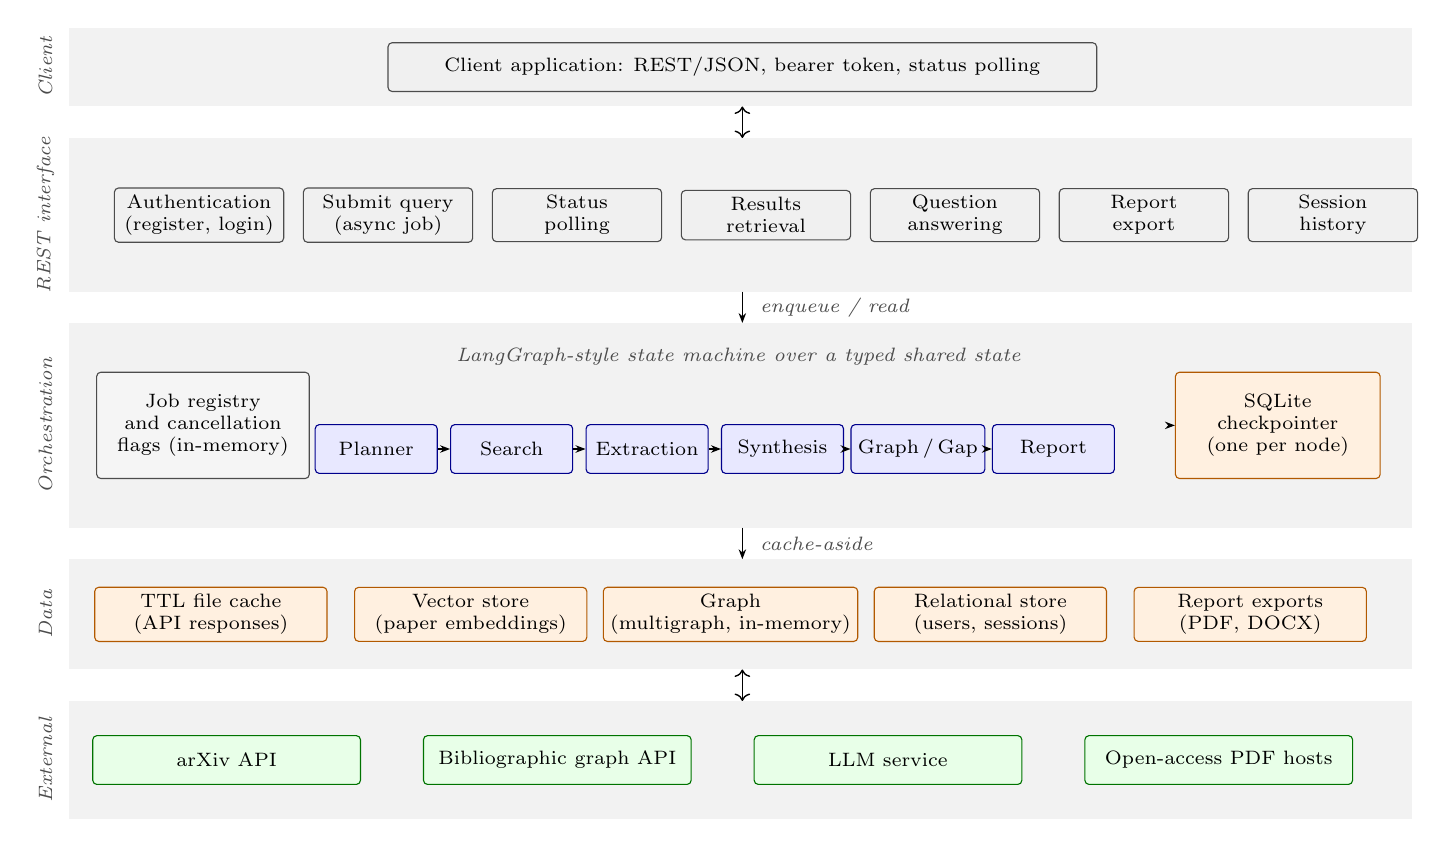
\begin{tikzpicture}[x=1cm,y=1cm]
% bands
\fill[band] (0.55,8.0) rectangle (17.6,9.0);
\fill[band] (0.55,5.65) rectangle (17.6,7.6);
\fill[band] (0.55,2.65) rectangle (17.6,5.25);
\fill[band] (0.55,0.85) rectangle (17.6,2.25);
\fill[band] (0.55,-1.05) rectangle (17.6,0.45);
\node[lab,rotate=90] at (0.25,8.5) {Client};
\node[lab,rotate=90] at (0.25,6.62) {REST interface};
\node[lab,rotate=90] at (0.25,3.95) {Orchestration};
\node[lab,rotate=90] at (0.25,1.55) {Data};
\node[lab,rotate=90] at (0.25,-0.3) {External};
% client
\node[apib,minimum width=9cm] (cl) at (9.1,8.5) {Client application: REST/JSON, bearer token, status polling};
% api row
\foreach \i/\t in {0/{Authentication\\(register, login)},1/{Submit query\\(async job)},2/{Status\\polling},3/{Results\\retrieval},4/{Question\\answering},5/{Report\\export},6/{Session\\history}}
  \node[apib,minimum width=2.15cm] (api\i) at (2.2+2.4*\i,6.62) {\t};
% orchestration
\node[blk,fill=gray!8,minimum width=2.7cm,minimum height=1.35cm] (jr) at (2.25,3.95) {Job registry\\and cancellation\\flags (in-memory)};
\begin{scope}[on background layer]
\node[draw=blue!55!black,dashed,rounded corners=3pt,fill=blue!3,minimum width=10.9cm,minimum height=2.15cm] (lg) at (9.05,3.95) {};
\end{scope}
\node[lab] at (9.05,4.82) {LangGraph-style state machine over a typed shared state};
\foreach \i/\t in {0/Planner,1/Search,2/Extraction,3/Synthesis,4/{Graph\,/\,Gap},5/Report}
  \node[agent,minimum width=1.55cm] (ag\i) at (4.45+1.72*\i,3.65) {\t};
\foreach \i/\j in {0/1,1/2,2/3,3/4,4/5} \draw[arr] (ag\i) -- (ag\j);
\node[dat,minimum width=2.6cm,minimum height=1.35cm] (ck) at (15.9,3.95) {SQLite\\checkpointer\\(one per node)};
\draw[darr] (lg.east) -- (ck.west);
% data
\foreach \i/\t in {0/{TTL file cache\\(API responses)},1/{Vector store\\(paper embeddings)},2/{Graph\\(multigraph, in-memory)},3/{Relational store\\(users, sessions)},4/{Report exports\\(PDF, DOCX)}}
  \node[dat,minimum width=2.95cm] (d\i) at (2.35+3.3*\i,1.55) {\t};
% external
\foreach \i/\t in {0/{arXiv API},1/{Bibliographic graph API},2/{LLM service},3/{Open-access PDF hosts}}
  \node[ext,minimum width=3.4cm] (e\i) at (2.55+4.2*\i,-0.3) {\t};
% vertical flows
\draw[arr,<->] (9.1,8.0) -- (9.1,7.6);
\draw[arr] (9.1,5.65) -- (9.1,5.25);
\draw[arr] (9.1,2.65) -- (9.1,2.25);
\draw[arr,<->] (9.1,0.85) -- (9.1,0.45);
\node[lab,anchor=west] at (9.2,5.45) {enqueue / read};
\node[lab,anchor=west] at (9.2,2.45) {cache-aside};
\end{tikzpicture}
\caption{Layered architecture of \RM. Dashed region: the orchestrated pipeline. Orange: stores. Green: external services.}
\label{fig:arch}
\end{figure*}

\subsection{Shared State and the Pipeline Function}
The pipeline state is the tuple
\begin{equation}
\cS=\langle q_0,\Phi,\cQ,\cP,\cF,\cZ,\cM,G,\Gamma,\cR,\alpha\rangle ,
\label{eq:state}
\end{equation}
where $q_0$ is the topic, $\Phi=(y_{\min},y_{\max})$ an optional year filter, $\cQ$ the sub-queries, $\cP$ the corpus, $\cF$ the field records, $\cZ$ the summaries, $\cM$ the comparison table, $G$ the graph, $\Gamma$ the gap claims, $\cR$ the report, and $\alpha:\mathcal{A}\to\{\textit{pending},\textit{running},\textit{done},\textit{error},\textit{cancelled}\}$ the per-agent status map over $\mathcal{A}=\{\text{plan},\text{search},\text{extract},\text{synth},\text{graph},\text{report}\}$. The pipeline is the composition
\begin{equation}
\cS_k=a_k(\cS_{k-1}),\quad k=1,\dots,6,
\label{eq:pipeline}
\end{equation}
where each agent $a_k$ reads a declared subset of $\cS$ and writes a disjoint subset (Table~\ref{tab:rw}). The disjoint write sets make the chain a pure data-flow: no agent overwrites another agent's output, so a checkpoint taken after $a_k$ is sufficient to restart at $a_{k+1}$.

\begin{table}[!t]
\caption{Data contract: fields read and written by each agent.}
\label{tab:rw}
\centering
\small
\begin{tabular}{@{}lll@{}}
\toprule
Agent & Reads & Writes \\
\midrule
Planner    & $q_0,\Phi$ & $\cQ$ \\
Search     & $\cQ,\Phi$ & $\cP$ (+ vector index) \\
Extraction & $\cP$ & $\cF$ \\
Synthesis  & $\cP,\cF$ & $\cZ,\cM$ \\
Graph/Gap  & $\cP$ & $G,\Gamma$ \\
Report     & $q_0,\cZ,\cM,\Gamma$ & $\cR$ \\
\bottomrule
\end{tabular}
\end{table}

\begin{figure*}[!t]
\centering
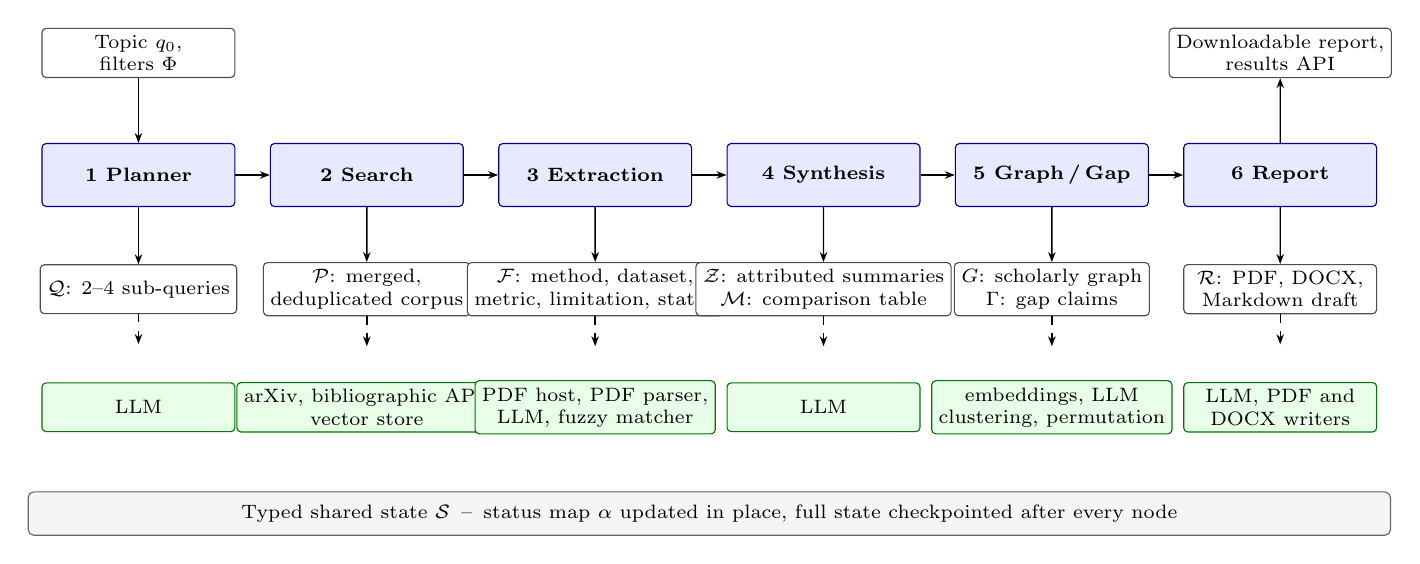
\begin{tikzpicture}[x=1cm,y=1cm]
\foreach \i/\t in {0/{1~Planner},1/{2~Search},2/{3~Extraction},3/{4~Synthesis},4/{5~Graph\,/\,Gap},5/{6~Report}}
  \node[agent,minimum width=2.45cm,minimum height=0.8cm] (a\i) at (1.45+2.9*\i,2.2) {\textbf{\t}};
\foreach \i/\j in {0/1,1/2,2/3,3/4,4/5} \draw[arr] (a\i) -- (a\j);
% artifacts
\node[blk,minimum width=2.45cm] (r0) at (1.45,0.75) {$\cQ$: 2--4 sub-queries};
\node[blk,minimum width=2.45cm] (r1) at (4.35,0.75) {$\cP$: merged,\\deduplicated corpus};
\node[blk,minimum width=2.45cm] (r2) at (7.25,0.75) {$\cF$: method, dataset,\\metric, limitation, status};
\node[blk,minimum width=2.45cm] (r3) at (10.15,0.75) {$\cZ$: attributed summaries\\$\cM$: comparison table};
\node[blk,minimum width=2.45cm] (r4) at (13.05,0.75) {$G$: scholarly graph\\$\Gamma$: gap claims};
\node[blk,minimum width=2.45cm] (r5) at (15.95,0.75) {$\cR$: PDF, DOCX,\\Markdown draft};
\foreach \i in {0,...,5} \draw[arr] (a\i.south) -- (r\i.north);
% dependencies
\node[ext,minimum width=2.45cm] at (1.45,-0.75) {LLM};
\node[ext,minimum width=2.45cm] at (4.35,-0.75) {arXiv, bibliographic API,\\vector store};
\node[ext,minimum width=2.45cm] at (7.25,-0.75) {PDF host, PDF parser,\\LLM, fuzzy matcher};
\node[ext,minimum width=2.45cm] at (10.15,-0.75) {LLM};
\node[ext,minimum width=2.45cm] at (13.05,-0.75) {embeddings, LLM\\clustering, permutation};
\node[ext,minimum width=2.45cm] at (15.95,-0.75) {LLM, PDF and\\DOCX writers};
\foreach \i in {0,...,5} \draw[darr] (r\i.south) -- ++(0,-0.38);
% input / output
\node[blk,minimum width=2.45cm] (in) at (1.45,3.75) {Topic $q_0$,\\filters $\Phi$};
\draw[arr] (in) -- (a0);
\node[blk,minimum width=2.45cm] (out) at (15.95,3.75) {Downloadable report,\\results API};
\draw[arr] (a5) -- (out);
% state bar
\node[draw=black!60,fill=gray!8,minimum width=17.3cm,minimum height=0.55cm,font=\scriptsize,rounded corners=2pt] at (8.7,-2.1) {Typed shared state $\cS$ \,--\, status map $\alpha$ updated in place, full state checkpointed after every node};
\end{tikzpicture}
\caption{Pipeline overview. Solid arrows: control and data flow. Dashed arrows: external dependencies used by each stage.}
\label{fig:pipeline}
\end{figure*}

Fig.~\ref{fig:pipeline} summarises the data flow. Three runtime properties follow from the formulation.

\textbf{Checkpointing and resume.} The runtime persists $\cS_k$ after every node under a thread key equal to the job identifier. Invoking the compiled graph with a null input and the same key resumes from the last stored checkpoint; completed nodes are not re-run, and the interrupted node runs again, which gives at-least-once semantics for that node. The resume primitive exists in the implementation, but it is not yet bound to an endpoint.

\textbf{Live progress without a message bus.} Agents update $\alpha$ in place. Because the API layer holds a reference to the same status map, a polling client observes transitions while the graph is executing. We verified in a probe that in-place mutation of a nested map is visible to the holder of the reference during execution (Section~\ref{sec:eval}-E).

\textbf{Job lifecycle.} A job and each agent follow the state machines of Fig.~\ref{fig:states}. An agent may record \textit{error} and still hand a fallback value to its successor (e.g., the planner falls back to $\cQ=\{q_0\}$), so \textit{error} at the agent level does not imply job failure.

\begin{figure*}[!t]
\centering
\begin{minipage}[t]{0.48\textwidth}
\centering
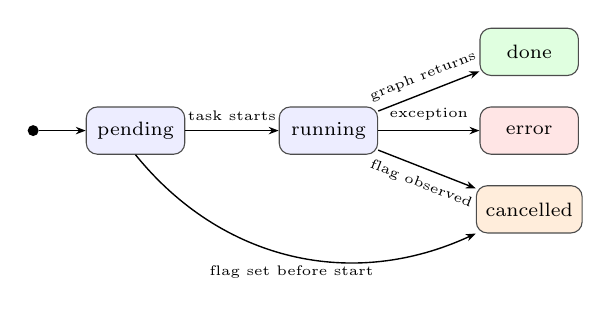
\begin{tikzpicture}[x=1cm,y=1cm]
\node[circle,fill=black,inner sep=1.4pt] (i0) at (-0.2,0) {};
\node[st] (pe) at (1.1,0) {pending};
\node[st] (ru) at (3.55,0) {running};
\node[st,fill=green!12] (dn) at (6.1,1.0) {done};
\node[st,fill=red!10] (er) at (6.1,0) {error};
\node[st,fill=orange!14] (ca) at (6.1,-1.0) {cancelled};
\draw[arr] (i0) -- (pe);
\draw[arr] (pe) -- node[above,font=\tiny]{task starts} (ru);
\draw[arr] (ru) -- node[above,sloped,font=\tiny]{graph returns} (dn);
\draw[arr] (ru) -- node[above,font=\tiny]{exception} (er);
\draw[arr] (ru) -- node[below,sloped,font=\tiny]{flag observed} (ca);
\draw[arr] (pe.south) to[bend right=38] node[below,font=\tiny]{flag set before start} (ca.south west);
\end{tikzpicture}

\small (a) Job lifecycle
\end{minipage}\hfill
\begin{minipage}[t]{0.48\textwidth}
\centering
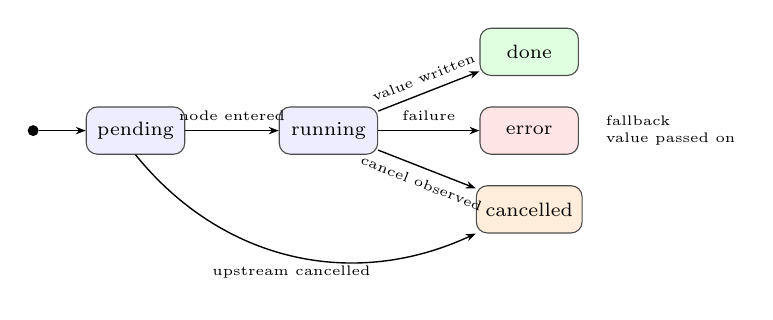
\begin{tikzpicture}[x=1cm,y=1cm]
\node[circle,fill=black,inner sep=1.4pt] (i0) at (-0.2,0) {};
\node[st] (pe) at (1.1,0) {pending};
\node[st] (ru) at (3.55,0) {running};
\node[st,fill=green!12] (dn) at (6.1,1.0) {done};
\node[st,fill=red!10] (er) at (6.1,0) {error};
\node[st,fill=orange!14] (ca) at (6.1,-1.0) {cancelled};
\draw[arr] (i0) -- (pe);
\draw[arr] (pe) -- node[above,font=\tiny]{node entered} (ru);
\draw[arr] (ru) -- node[above,sloped,font=\tiny]{value written} (dn);
\draw[arr] (ru) -- node[above,font=\tiny]{failure} (er);
\draw[arr] (ru) -- node[below,sloped,font=\tiny]{cancel observed} (ca);
\draw[arr] (pe.south) to[bend right=38] node[below,font=\tiny]{upstream cancelled} (ca.south west);
\node[font=\tiny,align=left,anchor=west] at (6.95,0) {fallback\\value passed on};
\end{tikzpicture}

\small (b) Per-agent status
\end{minipage}
\caption{State machines. (a) The job as seen by the API. (b) Each agent's entry in $\alpha$; downstream agents short-circuit to \textit{cancelled} when an upstream agent was cancelled.}
\label{fig:states}
\end{figure*}

\subsection{Data Model}
Four record types carry the stage outputs (Table~\ref{tab:records}). A paper record carries both a canonical identifier (DOI where available, otherwise an arXiv or bibliographic-service identifier) and the raw fields needed for merging. A field record carries a verification status and an abstract-only flag so that consumers can tell grounded fields from inferred ones. Records are validated by a typed schema at construction time, which rejects malformed LLM or API output before it enters the shared state.

\begin{table}[!t]
\caption{Core records. Fields marked $\dagger$ drive downstream decisions.}
\label{tab:records}
\centering
\small
\begin{tabular}{@{}p{1.55cm}p{6.35cm}@{}}
\toprule
Record & Fields \\
\midrule
Paper & id, title, authors, year, venue, abstract, PDF URL, page URL, DOI, arXiv id, citation count, citation list$^\dagger$, full-text flag$^\dagger$, source $\in\{$arXiv, bibliographic API, merged$\}$ \\
Field record & paper id, method, dataset, key metric, limitation, year, verification status$^\dagger\in\{$verified, unverified, failed, heuristic$\}$, notes, abstract-only flag$^\dagger$ \\
Summary & paper id, title, summary text, sentence-level attributions \\
Gap claim & gap id, topic label, description, citation density, member paper ids, induced-subgraph snapshot, suggested directions, signal-degraded flag \\
\bottomrule
\end{tabular}
\end{table}
\section{Pipeline Stages}
\label{sec:stages}

\subsection{Query Planning}
The planner issues one LLM call at temperature $0$ asking for between two and four distinct, highly specific search queries, each covering a different facet, methodology, or angle of the topic, and returned as a bare JSON array. The reply is stripped of code fences, parsed, cast to strings, and filtered for empty entries:
\begin{equation}
\cQ=\begin{cases}\mathrm{Parse}\big(\mathrm{LLM}(q_0,\Phi)\big) & \text{if valid and non-empty},\\ \{q_0\} & \text{otherwise.}\end{cases}
\label{eq:plan}
\end{equation}
On failure the planner records \textit{error} but does not abort (Fig.~\ref{fig:states}b). Decomposition diversifies retrieval: each sub-query ranks the two sources differently, so the union covers facets that a single query would rank below the per-source limit.

\subsection{Retrieval, Deduplication, and Merging}
\textbf{Retrieval.} Each sub-query is issued to two sources with a per-source limit $k=15$. The arXiv query matches the sub-query against title or abstract and, when a year filter is present, conjoins a submission-date range (missing bounds default to 1900 and 2099); results are sorted by relevance and re-filtered client-side. The bibliographic API is queried with its relevance ranking, the same year range, and a field list covering authors, venue, abstract, external identifiers, citation count, citation list, and open-access PDF link. The $2m$ calls ($m=|\cQ|$) run concurrently on a bounded pool of six workers, so the raw candidate set satisfies
\begin{equation}
\mathcal{R}=\bigcup_{q\in\cQ}\big(\mathrm{Arx}(q)\cup\mathrm{Bib}(q)\big),\qquad |\mathcal{R}|\le 2km\le 120 .
\label{eq:raw}
\end{equation}
A failed call is logged and skipped, so retrieval degrades to a partial corpus rather than failing.

\textbf{Duplicate predicate.} Let $t$ denote a title, $\kappa(t)$ its lower-cased alphanumeric-only form, $W(t)$ its set of lower-cased word tokens, and
\begin{equation}
J(t,t')=\frac{|W(t)\cap W(t')|}{|W(t)\cup W(t')|}
\label{eq:jaccard}
\end{equation}
the Jaccard coefficient \cite{jaccard1912}. A candidate $r$ duplicates an accepted record $e$ if
\begin{align}
\mathrm{dup}(r,e)\;=\;&[\mathrm{doi}_r=\mathrm{doi}_e]\;\lor\;[\mathrm{ax}_r=\mathrm{ax}_e]\nonumber\\
&\lor\;[\kappa(t_r)=\kappa(t_e)]\;\lor\;[J(t_r,t_e)\ge\tau_J],
\label{eq:dup}
\end{align}
with $\tau_J=0.8$; identifier tests apply only when both identifiers are present and are case-insensitive. The three tiers therefore run from exact identifiers, through exact normalised title, to approximate title.

\textbf{Merge operator.} On a match, the first-seen record is kept and enriched: missing DOI, arXiv identifier, and PDF link are filled; the full-text flag is OR-ed; the citation count becomes the maximum of the two; the citation list is copied only if the kept record has none; and the source label becomes \emph{merged} when the sources differ. Finally, ``title. abstract'' documents of the surviving papers are added to the vector store; an indexing failure is logged and does not stop the pipeline. Algorithm~\ref{alg:search} gives the procedure. The pairwise scan costs $O(|\mathcal{R}|\,|\cP|)$ title comparisons, at most a few thousand for $|\mathcal{R}|\le120$.

\begin{algorithm}[!t]
\caption{Retrieval, deduplication, and merge}
\label{alg:search}
\small
\begin{algorithmic}[1]
\Require sub-queries $\cQ$, filter $\Phi$, limit $k$, threshold $\tau_J$
\Ensure corpus $\cP$
\State $\mathcal{R}\gets\emptyset$
\ForAll{$(s,q)\in\{\text{Arx},\text{Bib}\}\times\cQ$ \textbf{in parallel}}
  \State $\mathcal{R}\gets\mathcal{R}\cup\textsc{Search}_s(q,k,\Phi)$ \Comment{cache, then API}
  \Statex \hspace{1.3em}\textit{(on failure: log, continue)}
\EndFor
\If{job cancelled} \State \Return $\emptyset$ \EndIf
\State $\cP\gets[\,]$
\ForAll{$r\in\mathcal{R}$}
  \State $e\gets$ first $e\in\cP$ with $\mathrm{dup}(r,e)$
  \If{$e$ exists} \State $\textsc{Merge}(e,r)$
  \Else \State append $r$ to $\cP$ \EndIf
\EndFor
\State index $\{\text{title}\Vert\text{abstract}\}$ of $\cP$ in vector store
\State \Return $\cP$
\end{algorithmic}
\end{algorithm}

\subsection{Structured Extraction and Grounding Verification}
For every paper the extraction agent produces a field record $f_p=(m,d,\mu,\ell,\sigma)$ holding the proposed method, evaluation dataset, key metric, limitation, and a verification status $\sigma$. Papers are processed concurrently by eight workers into index-addressed slots, which preserves the corpus order. The per-paper cascade of Fig.~\ref{fig:extract} and Algorithm~\ref{alg:extract} has four stages.

\textbf{(1) Text acquisition.} If a PDF link exists and the full-text flag is set, the PDF is downloaded with a 20-second timeout; the payload must begin with the PDF magic bytes. Text is extracted from the first four and last two pages (all pages when there are six or fewer), which balances coverage of the abstract and method against the results and limitation sections.

\textbf{(2) Prompted extraction.} In full-text mode the prompt contains the first $12{,}000$ characters of text and requires, for each field, a value and a short supporting quotation. In abstract-only mode the prompt contains the title and abstract and requires values only. Both run at temperature $0$ and return JSON, which is parsed tolerantly (fences, preambles, and surrounding prose are stripped).

\textbf{(3) Second-pass inference.} A field is \emph{blank} if it is empty, shorter than five characters, or a stock phrase such as ``not available''. If $B\ne\emptyset$ blank fields remain, one further call at temperature $0.1$ asks targeted questions for only those fields, using the title and abstract.

\textbf{(4) Verification.} Let $\nu(\cdot)$ denote the normalisation that applies Unicode NFKC, removes page markers, rejoins hyphenated line breaks, unifies quotation marks and dashes, collapses whitespace, and lower-cases. For a quote $u$ with $m=|\nu(u)|$ characters and a text $T$, the match score is
\begin{equation}
\rho(u,T)=\begin{cases}1 & \nu(u)\ \text{occurs in}\ \nu(T),\\[2pt] \max_{i}\ r_i(u,T) & \text{otherwise,}\end{cases}
\label{eq:rho}
\end{equation}
where $r_i(u,T)=2M/(2m)$ compares $\nu(u)$ with the window $\nu(T)_{[i,i+m)}$ and $i$ runs over multiples of the stride $s=\max(\lfloor m/4\rfloor,20)$. Here $M$ is the number of matching characters found by gestalt pattern matching \cite{ratcliff1988gestalt}, i.e., recursive longest-common-block matching, so $r_i$ is the standard similarity ratio. The status of field $f$ with value $x_f$ and quote $u_f$ is
\begin{equation}
\sigma_f=\begin{cases}
\textit{verified} & x_f\ \text{empty or ``not specified''},\\
\textit{unverified} & u_f\ \text{absent},\\
\textit{verified} & \rho(u_f,T)\ge 0.85,\\
\textit{unverified} & 0.5\le\rho(u_f,T)<0.85,\\
\textit{failed} & \rho(u_f,T)<0.5,
\end{cases}
\label{eq:sigmaf}
\end{equation}
and the record status aggregates the worst case,
\begin{equation}
\sigma=\begin{cases}
\textit{failed} & \exists f:\sigma_f=\textit{failed},\\
\textit{verified} & \forall f:\sigma_f=\textit{verified},\\
\textit{unverified} & \text{otherwise.}
\end{cases}
\label{eq:sigma}
\end{equation}
In abstract-only mode there is no quote to locate, so the check is weaker: $\sigma_f=\textit{verified}$ iff a number in $x_f$ occurs in $T=\text{title}\,\Vert\,\text{abstract}$ or at least two significant words of $x_f$ (length $\ge4$, outside a small stop list) occur in $T$; otherwise \textit{unverified}. Abstract-only records therefore can never be \textit{failed}, and they are additionally flagged as abstract-only.

\textbf{Heuristic fallback.} If an LLM call or the parse raises an exception, the record is built from curated keyword lists (architectures, benchmark names, task phrases) and regular expressions for numeric results and limitation cues applied to the title and abstract, and is labelled $\sigma=\textit{heuristic}$. The function never raises, so one failing paper cannot abort the stage. A paper costs one LLM call, or two if a second pass is needed; the dominant local cost is the sliding-window match, $O\!\big((|T|/s)\cdot c(m)\big)$ per quote where $c(m)$ is the cost of one gestalt comparison of length $m$.

\begin{algorithm}[!t]
\caption{Grounded extraction for one paper}
\label{alg:extract}
\small
\begin{algorithmic}[1]
\Require paper $p$
\Ensure field record $f_p$
\State $T\gets\emptyset$;\ \ mode $\gets$ \textsc{abstract-only}
\If{$p$ has PDF link \textbf{and} full-text flag}
  \State $b\gets\textsc{Get}(p.\text{pdf},\,20\text{ s})$
  \If{$b$ starts with \texttt{\%PDF}}
    \State $T\gets\textsc{Text}(b,\text{first 4 + last 2 pages})$
    \If{$T\ne\emptyset$} mode $\gets$ \textsc{full-text} \EndIf
  \EndIf
\EndIf
\State $\mathrm{ctx}\gets T[{:}12000]$ if full-text, else (title, abstract)
\State $x\gets\textsc{ParseJSON}\big(\textsc{LLM}(\text{prompt}_{\text{mode}},\mathrm{ctx},\tau{=}0)\big)$
\State $B\gets\{f:\textsc{Blank}(x_f)\}$
\If{$B\ne\emptyset$}
  \State $x_B\gets\textsc{LLM}(\text{targeted questions for }B,\,\tau{=}0.1)$
\EndIf
\State $(\sigma,\text{notes})\gets\textsc{Verify}(x,\,T\text{ or title}\Vert\text{abstract},\,\text{mode})$
\State \Return $(x,\sigma)$
\Statex \textit{on any exception above:}\ \Return \textsc{Heuristic}$(p)$ with $\sigma=\textit{heuristic}$
\end{algorithmic}
\end{algorithm}

\begin{figure*}[!t]
\centering
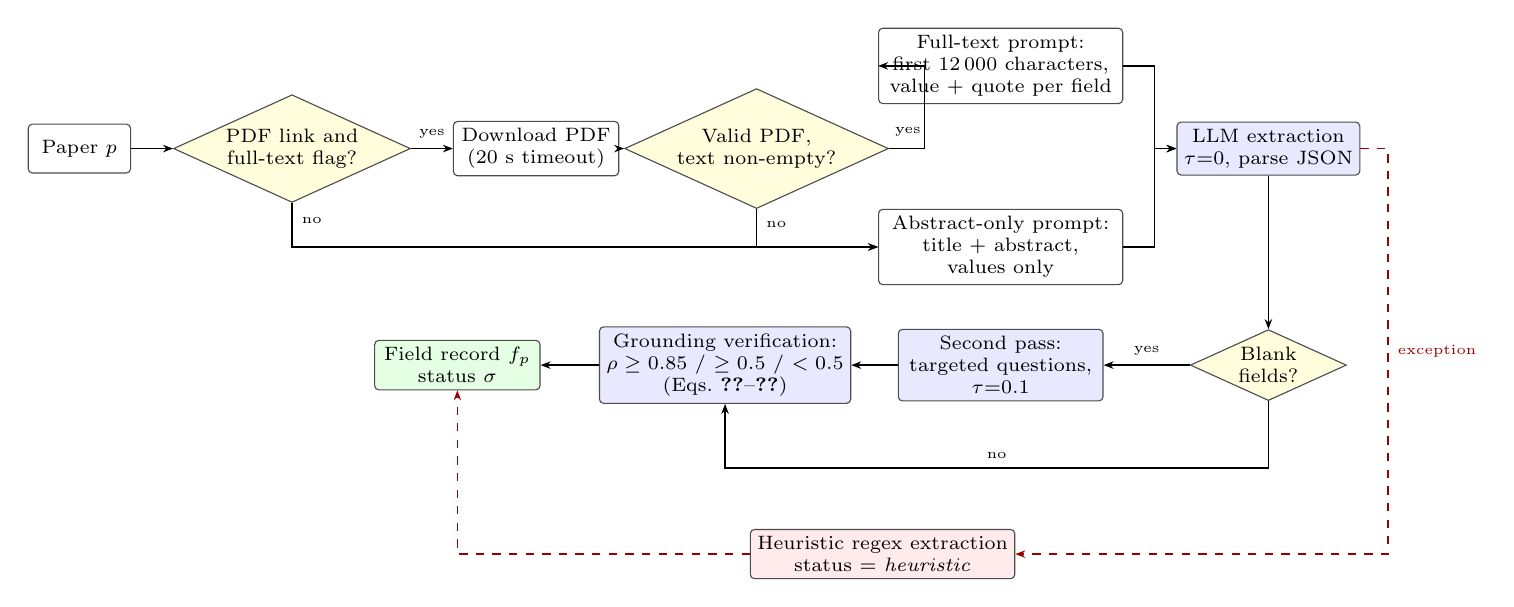
\begin{tikzpicture}[x=1cm,y=1cm]
\node[blk,minimum width=1.3cm] (n0) at (0.8,2.3) {Paper $p$};
\node[dia] (d1) at (3.5,2.3) {PDF link and\\full-text flag?};
\node[blk,minimum width=2.1cm] (n1) at (6.6,2.3) {Download PDF\\(20 s timeout)};
\node[dia] (d2) at (9.4,2.3) {Valid PDF,\\text non-empty?};
\node[blk,minimum width=3.1cm] (n2) at (12.5,3.35) {Full-text prompt:\\first 12\,000 characters,\\value + quote per field};
\node[blk,minimum width=3.1cm] (n3) at (12.5,1.05) {Abstract-only prompt:\\title + abstract,\\values only};
\node[blk,minimum width=2.1cm,fill=blue!9] (n4) at (15.9,2.3) {LLM extraction\\$\tau{=}0$, parse JSON};
\node[dia] (d3) at (15.9,-0.45) {Blank\\fields?};
\node[blk,minimum width=2.6cm,fill=blue!9] (n5) at (12.5,-0.45) {Second pass:\\targeted questions,\\$\tau{=}0.1$};
\node[blk,minimum width=2.7cm,fill=blue!9] (n6) at (9.0,-0.45) {Grounding verification:\\$\rho\ge0.85$ / $\ge0.5$ / $<0.5$\\(Eqs.~\ref{eq:rho}--\ref{eq:sigma})};
\node[blk,minimum width=2.1cm,fill=green!10] (n7) at (5.6,-0.45) {Field record $f_p$\\status $\sigma$};
\node[blk,minimum width=3.0cm,fill=red!8] (n8) at (11.0,-2.85) {Heuristic regex extraction\\status $=$ \textit{heuristic}};
\draw[arr] (n0) -- (d1);
\draw[arr] (d1) -- node[above,font=\tiny]{yes} (n1);
\draw[arr] (n1) -- (d2);
\draw[arr] (d2.east) -- ++(0.45,0) |- (n2.west);
\node[font=\tiny,anchor=south] at ($(d2.east)+(0.24,0.03)$) {yes};
\draw[arr] (d1.south) |- node[pos=0.2,right,font=\tiny]{no} (n3.west);
\draw[arr] (d2.south) |- node[pos=0.2,right,font=\tiny]{no} (n3.west);
\draw[arr] (n2.east) -- ++(0.4,0) |- (n4.west);
\draw[arr] (n3.east) -- ++(0.4,0) |- (n4.west);
\draw[arr] (n4) -- (d3);
\draw[arr] (d3) -- node[above,font=\tiny]{yes} (n5);
\draw[arr] (n5) -- (n6);
\draw[arr] (d3.south) -- ++(0,-0.85) -| node[pos=0.25,above,font=\tiny]{no} (n6.south);
\draw[arr] (n6) -- (n7);
\draw[darr,red!60!black] (n4.east) -- ++(0.35,0) -- ++(0,0) |- node[pos=0.25,right,font=\tiny,text=red!60!black]{exception} (n8.east);
\draw[darr,red!60!black] (n8.west) -| (n7.south);
\end{tikzpicture}
\caption{Per-paper extraction cascade. Dashed red path: any LLM or parsing exception routes to the rule-based fallback.}
\label{fig:extract}
\end{figure*}

\subsection{Attributed Synthesis}
For each paper one LLM call (temperature $0$) writes a three-sentence factual summary from the title, abstract, and extracted fields, and must end every sentence with a tag from $\{$Abstract, Method, Dataset, Key Metric, Limitation$\}$. A regular expression splits the output into sentences and captures the tag, yielding $(\text{sentence},\text{source})$ pairs; untagged sentences receive the label \emph{General Context}. On failure the summary text states the error explicitly rather than inventing content. The comparison-table row $\mathrm{row}_p$ is built deterministically from the paper and its field record, together with the verification status and the abstract-only flag, and a single resolver picks the most human-readable link in the order: explicit page URL, arXiv abstract page, DOI resolver, PDF link. Summaries are produced by eight concurrent workers into index-addressed slots.

\subsection{Graph Construction and Research Gap Detection}
\label{sec:gap}
This stage turns the corpus into a heterogeneous graph, groups papers into thematic clusters, and flags clusters whose citation and similarity structure is unusual relative to a permutation null.

\textbf{Corpus gate.} Gap detection requires clusters with enough members to estimate densities; when $|\cP|<15$ the stage returns $\Gamma=\emptyset$ and $G=\varnothing$ and records \textit{done}.

\textbf{Graph.} The graph is a typed multi-digraph $G=(V,E)$ with $V=V_P\cup V_A\cup V_T$ (papers, authors, topics; Fig.~\ref{fig:graph}). Let $A_p$ be the authors, $L_p$ the citation list, and $e_p$ the embedding of paper $p$. With
\begin{equation}
\mathrm{sim}(p,q)=\frac{e_p^{\top}e_q}{\lVert e_p\rVert\,\lVert e_q\rVert},
\label{eq:cos}
\end{equation}
and the similarity threshold $\tau_s=0.6$, the edge sets are
\begin{align}
E_{\mathrm{auth}}&=\{(p,a):a\in A_p\},\nonumber\\
E_{\mathrm{co}}&=\{(a,a'),(a',a):a\neq a'\in A_p,\ p\in\cP\},\nonumber\\
E_{\mathrm{cite}}&=\{(p,q):q\in L_p\cap\mathrm{ids}(\cP)\},\nonumber\\
E_{\mathrm{sim}}&=\{(p,q),(q,p):\mathrm{sim}(p,q)\ge\tau_s\},\nonumber\\
E_{\mathrm{bel}}&=\{(p,T_k):p\in C_k\}.
\label{eq:edges}
\end{align}
Citation edges are restricted to targets inside the corpus, so they encode intra-corpus influence only. Co-authorship is stored as a pair of opposite directed edges per shared paper (parallel edges for repeated collaboration). Embeddings come from the vector store's default sentence-embedding function \cite{reimers2019sbert}; all pairwise cosines are obtained with one normalised matrix product, $\hat E\hat E^{\top}$, where $\hat E$ has unit-norm rows. If the embedding model cannot be loaded, the store substitutes deterministic pseudo-random $384$-dimensional unit vectors seeded by a hash of the text, and the graph is flagged \emph{embeddings-degraded}. For independent random unit vectors in $\mathbb{R}^{384}$ the cosine has standard deviation $1/\sqrt{384}\approx0.051$, so $\tau_s=0.6$ lies about $11.8\sigma$ away and essentially no similarity edges are created in the degraded mode. Algorithm~\ref{alg:graph} summarises construction.

\begin{algorithm}[!t]
\caption{Heterogeneous graph construction}
\label{alg:graph}
\small
\begin{algorithmic}[1]
\Require corpus $\cP$, embedding store, $\tau_s$
\Ensure multi-digraph $G$
\ForAll{$p\in\cP$}
  \State add Paper node $p$ (title, year, venue, \dots)
  \ForAll{$a\in A_p$}
     \State add Author node $a$;\ add $(p,a)$ \textsc{authored\_by}
  \EndFor
  \ForAll{unordered pairs $\{a,a'\}\subseteq A_p$}
     \State add $(a,a')$ and $(a',a)$ \textsc{co\_authored\_with}
  \EndFor
  \ForAll{$q\in L_p$ with $q\in\mathrm{ids}(\cP)$}
     \State add $(p,q)$ \textsc{cites}
  \EndFor
\EndFor
\State $U\gets\{p: e_p\ \text{available}\}$;\ \ $S\gets\hat E\hat E^{\top}$
\ForAll{$p<q$ in $U$ with $S_{pq}\ge\tau_s$}
  \State add $(p,q),(q,p)$ \textsc{similar\_topic}, weight $S_{pq}$
\EndFor
\State \Return $G$
\end{algorithmic}
\end{algorithm}

\begin{figure}[!t]
\centering
\resizebox{\columnwidth}{!}{%
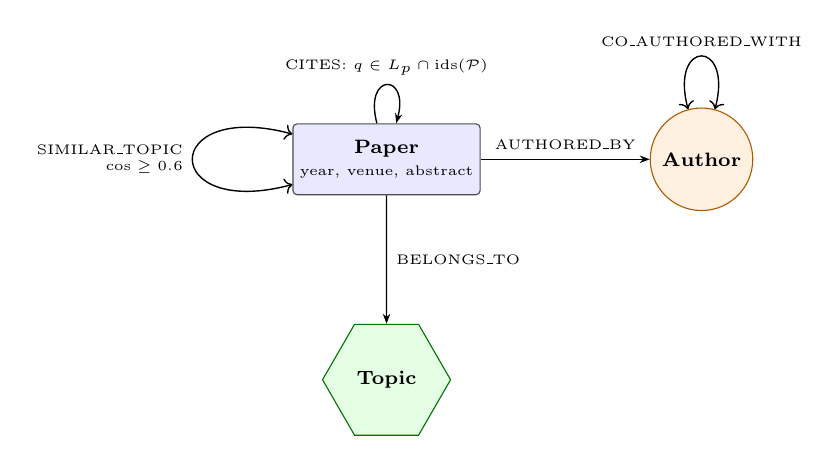
\begin{tikzpicture}[x=1cm,y=1cm]
\node[blk,minimum width=2.0cm,minimum height=0.9cm,fill=blue!9] (P) at (3.6,1.3) {\textbf{Paper}\\\tiny year, venue, abstract};
\node[circle,draw=orange!70!black,fill=orange!12,minimum size=1.05cm,font=\scriptsize,line width=0.4pt] (A) at (7.6,1.3) {\textbf{Author}};
\node[regular polygon,regular polygon sides=6,draw=green!45!black,fill=green!10,minimum size=1.15cm,font=\scriptsize,line width=0.4pt] (T) at (3.6,-1.5) {\textbf{Topic}};
\draw[arr] (P) -- node[above,font=\tiny]{AUTHORED\_BY} (A);
\draw[arr] (P) -- node[right,font=\tiny]{BELONGS\_TO} (T);
\path (P) edge[arr,loop above,looseness=7] node[above,font=\tiny,align=center]{CITES: $q\in L_p\cap\mathrm{ids}(\cP)$} (P);
\path (P) edge[arr,<->,loop left,looseness=7] node[left,font=\tiny,align=right]{SIMILAR\_TOPIC\\$\cos\ge0.6$} (P);
\path (A) edge[arr,<->,loop above,looseness=7] node[above,font=\tiny,align=center]{CO\_AUTHORED\_WITH} (A);
\end{tikzpicture}}
\caption{Schema of the scholarly graph. Double-headed edges are stored as two opposite directed edges.}
\label{fig:graph}
\end{figure}

\textbf{Topic clustering.} One LLM call receives the identifier, title, and first 300 characters of the abstract of every paper and returns three to five thematic clusters $\cC=\{C_1,\dots,C_K\}$, each with a label, a one-sentence description, and member identifiers; every paper is requested to appear at least once, and clusters may overlap. Identifiers not in the corpus are dropped. If the call or parse fails, a keyword-based fallback assigns each paper to the cluster of the first matching entry in a nine-term vocabulary, with a catch-all cluster for the remainder. Topic nodes and membership edges $E_{\mathrm{bel}}$ are then added to $G$.

\textbf{Signal 1: age-adjusted citation pace.} Let $Y$ be the current calendar year, $y_p$ the publication year of $p$, and $\deg^{-}_{\mathrm{cite}}(p)$ the number of in-corpus citation edges into $p$. The pace of cluster $k$ is
\begin{equation}
\pi_k=\frac{\sum_{p\in C_k}\deg^{-}_{\mathrm{cite}}(p)}{\max\!\Big(1,\ \sum_{p\in C_k}\max(1,\,Y-y_p)\Big)} .
\label{eq:pace}
\end{equation}
It is a citations-per-paper-year rate: dividing by accumulated paper age prevents older clusters from appearing better cited merely because they have had longer to accumulate citations \cite{wang2013quantifying}.

\textbf{Signal 2: cross-cluster bridge strength.} Let $w_k$ be the number of similarity edges inside $C_k$ and $b_{kl}$ the number crossing between $C_k$ and $C_l$:
\begin{align}
w_k&=\big|E_{\mathrm{sim}}\cap(C_k\times C_k)\big|,\nonumber\\
b_{kl}&=\big|E_{\mathrm{sim}}\cap\big((C_k\times C_l)\cup(C_l\times C_k)\big)\big|.
\label{eq:wb}
\end{align}
The bridge strength of cluster $k$ is its weakest normalised connection to any other cluster,
\begin{equation}
\beta_k=\min_{l\neq k}\ \frac{b_{kl}}{w_k+w_l+1},\qquad \beta_k=0\ \text{if}\ K=1 .
\label{eq:bridge}
\end{equation}
The $+1$ smooths empty clusters. Because the minimum is taken over \emph{all} other clusters, $\beta_k$ is large only if cluster $k$ is similar to every other cluster.

\textbf{Gap score.} Both signals are min--max normalised across clusters, with the all-equal case mapped to zero,
\begin{equation}
\norm{x}_k=\begin{cases}\dfrac{x_k-\min_j x_j}{\max_j x_j-\min_j x_j} & \max_j x_j>\min_j x_j,\\[4pt] 0 & \text{otherwise,}\end{cases}
\label{eq:minmax}
\end{equation}
and combined as
\begin{equation}
s_k=\norm{\beta}_k-\norm{\pi}_k\ \in[-1,1].
\label{eq:score}
\end{equation}
A high score therefore means: lightly cited for its age \emph{and} strongly bridged to the rest of the corpus, i.e. an under-cited junction between themes (note the sign: larger $\beta_k$ raises $s_k$).

\textbf{Permutation calibration.} A raw score has no natural scale, so it is compared with a null in which cluster membership carries no structure. For $r=1,\dots,R$ ($R=100$) the paper identifiers are randomly re-partitioned into clusters of the original sizes, the scores $s^{(r)}_1,\dots,s^{(r)}_K$ are recomputed with the same formulas on the same graph, and all $RK$ values are pooled into $\mathcal{N}$. The threshold is the $90$th percentile of the pooled null (linear interpolation),
\begin{equation}
\theta=\Quant_{0.90}(\mathcal{N}),\qquad \Gamma=\{k:\ s_k\ge\theta\}.
\label{eq:theta}
\end{equation}
Under the null each real score is approximately a draw from $\mathcal{N}$, so each cluster is flagged with probability close to $0.10$. The test is applied once per cluster without multiplicity correction, and with finite $R$ the quantile is itself estimated \cite{efron1979bootstrap,phipson2010permutation}. The inequality in Eq.~\eqref{eq:theta} is non-strict, which matters when scores tie (Section~\ref{sec:eval}-D). Algorithm~\ref{alg:gap} and Fig.~\ref{fig:gapflow} summarise the computation. Counting similarity edges for all cluster pairs costs $O(K^2|E_{\mathrm{sim}}|)$ per replicate, hence $O(RK^2|E_{\mathrm{sim}}|)$ overall, which is negligible at corpus sizes of a few hundred papers.

\begin{algorithm}[!t]
\caption{Bootstrap-calibrated gap detection}
\label{alg:gap}
\small
\begin{algorithmic}[1]
\Require graph $G$, clusters $\cC$, year $Y$, $R=100$, $q=0.90$
\Ensure gap claims $\Gamma$
\Function{Score}{$\cC$}
  \State $\pi_k\gets$ Eq.~\eqref{eq:pace};\ \ $\beta_k\gets$ Eq.~\eqref{eq:bridge}
  \State \Return $\norm{\beta}-\norm{\pi}$ \Comment{Eqs.~\eqref{eq:minmax},\eqref{eq:score}}
\EndFunction
\State $s\gets\textsc{Score}(\cC)$;\ \ $\mathcal{N}\gets\emptyset$
\For{$r=1$ \textbf{to} $R$}
  \State $\cC^{(r)}\gets$ random partition of paper ids, sizes $|C_k|$
  \State $\mathcal{N}\gets\mathcal{N}\cup\textsc{Score}(\cC^{(r)})$
\EndFor
\State $\theta\gets\Quant_q(\mathcal{N})$;\ \ $\Gamma\gets\emptyset$
\For{$k=1$ \textbf{to} $K$ \textbf{with} $s_k\ge\theta$}
  \State $\Gamma\gets\Gamma\cup\textsc{Claim}(k,\pi_k,\beta_k)$
\EndFor
\State \Return $\Gamma$
\end{algorithmic}
\end{algorithm}

\begin{figure*}[!t]
\centering
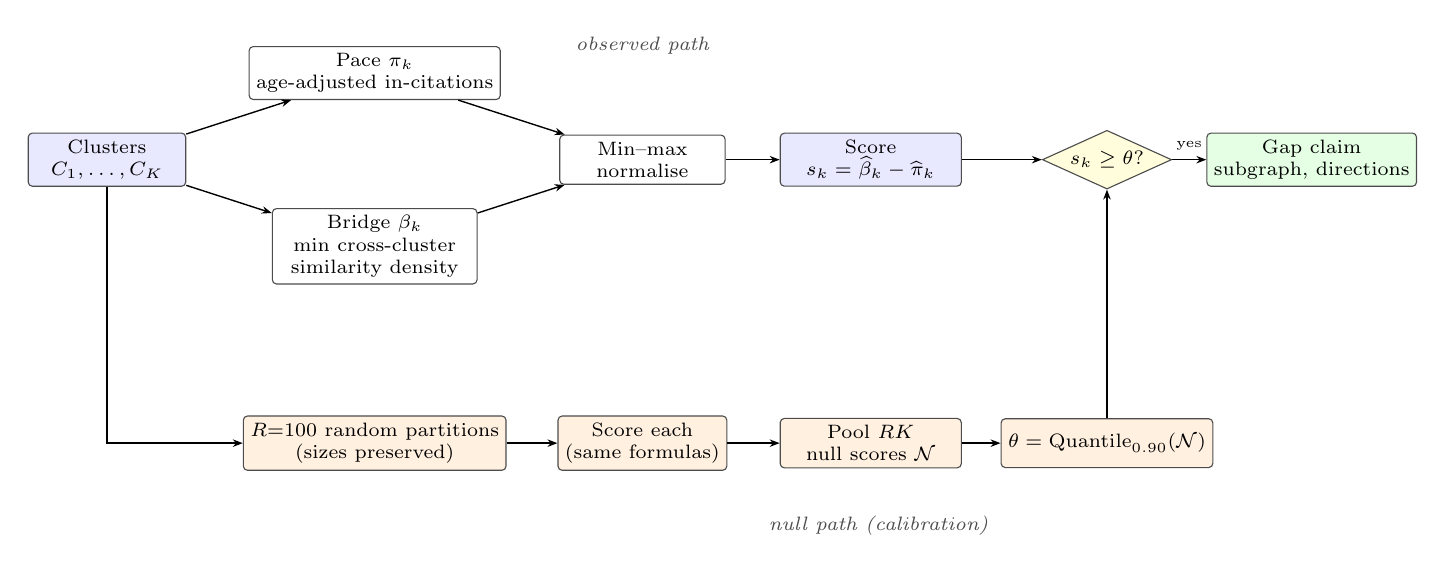
\begin{tikzpicture}[x=1cm,y=1cm]
\node[blk,minimum width=2.0cm,fill=blue!9] (cl) at (1.2,1.9) {Clusters\\$C_1,\dots,C_K$};
\node[blk,minimum width=2.6cm] (pi) at (4.6,3.0) {Pace $\pi_k$\\age-adjusted in-citations};
\node[blk,minimum width=2.6cm] (be) at (4.6,0.8) {Bridge $\beta_k$\\min cross-cluster\\similarity density};
\node[blk,minimum width=2.1cm] (mm) at (8.0,1.9) {Min--max\\normalise};
\node[blk,minimum width=2.3cm,fill=blue!9] (sc) at (10.9,1.9) {Score\\$s_k=\norm{\beta}_k-\norm{\pi}_k$};
\node[dia] (dc) at (13.9,1.9) {$s_k\ge\theta$?};
\node[blk,minimum width=2.1cm,fill=green!10] (gc) at (16.5,1.9) {Gap claim\\subgraph, directions};
\draw[arr] (cl) -- (pi); \draw[arr] (cl) -- (be);
\draw[arr] (pi) -- (mm); \draw[arr] (be) -- (mm);
\draw[arr] (mm) -- (sc); \draw[arr] (sc) -- (dc);
\draw[arr] (dc) -- node[above,font=\tiny]{yes} (gc);
% null path
\node[blk,minimum width=2.6cm,fill=orange!12] (rp) at (4.6,-1.7) {$R{=}100$ random partitions\\(sizes preserved)};
\node[blk,minimum width=2.1cm,fill=orange!12] (sn) at (8.0,-1.7) {Score each\\(same formulas)};
\node[blk,minimum width=2.3cm,fill=orange!12] (pl) at (10.9,-1.7) {Pool $RK$\\null scores $\mathcal{N}$};
\node[blk,minimum width=2.1cm,fill=orange!12] (th) at (13.9,-1.7) {$\theta=\Quant_{0.90}(\mathcal{N})$};
\draw[arr] (cl.south) |- (rp.west);
\draw[arr] (rp) -- (sn); \draw[arr] (sn) -- (pl); \draw[arr] (pl) -- (th);
\draw[arr] (th.north) -- (dc.south);
\node[lab] at (8.0,3.35) {observed path};
\node[lab] at (11.0,-2.75) {null path (calibration)};
\end{tikzpicture}
\caption{Computation of the gap score and its calibrated threshold. The null path re-scores random partitions of the same sizes on the same graph.}
\label{fig:gapflow}
\end{figure*}

\textbf{Gap claims.} For every flagged cluster the agent (i) extracts the induced subgraph on the member papers, their authors, and the topic node and serialises it as node-link JSON; (ii) stores $\pi_k$ as the claim's citation density; (iii) writes a description reporting $\pi_k$ and $\beta_k$ and stating that the score exceeds the null's 90th percentile; and (iv) proposes three template research directions (integrate with adjacent developments, validate on broader benchmarks, study scaling and deployment constraints), parameterised by a distinctive two-word phrase mined from member abstracts. If every cluster's pace is below $0.01$, the description instead warns that the corpus may be too recent to carry a meaningful citation signal; if embeddings are degraded, the claim is prefixed with a warning and its signal-degraded flag is set.

\subsection{Report Generation}
The report agent assembles four sections. The \emph{comparison matrix} is data-driven from $\cM$. Three sections are LLM-written at temperature $0.2$: the \emph{introduction} (two paragraphs motivating the topic, stating objectives, summarising the method, and outlining the structure), the \emph{thematic synthesis} (exactly four mandated subsections: methodological landscape; datasets, benchmarks and evaluation protocols; common limitations and open challenges; and critical assessment, conditioned on all summaries and gap claims), and one \emph{narrative paragraph per gap} of 120--180 words explaining why the gap exists, why it matters, and how a suggested direction could be pursued. The introduction and synthesis are generated concurrently by two workers, and gap narratives by up to five workers into index-addressed slots. Any failed section falls back to deterministic template text. The result is stored as a Markdown draft in the state, and the same content is rendered to a PDF and a DOCX document in an export store; a download endpoint streams the requested format.

\section{Question Answering over a Completed Review}
\label{sec:qa}
After a job completes, a user can ask questions about the retrieved literature. The service builds a bounded evidence set for the question and prompts the LLM with it. Selecting evidence is the interesting part, because questions mix three intents: referring to a specific paper (``explain paper 3''), naming one by title or author, and asking a topical question that should be answered across papers. Let $W_q$ be the question tokens longer than three characters outside a small stop list, and let $\mathrm{text}(p)$ be the lower-cased concatenation of title, abstract, method, and dataset. Candidates are collected in five stages of decreasing specificity, and a paper already selected is never added twice:
\begin{enumerate}
\item[\textbf{A}] \emph{Index reference.} A pattern such as ``paper $n$'', ``source $n$'', ``ref $n$'', or ``\#$n$'' selects the $n$-th paper of the session.
\item[\textbf{B}] \emph{Title or author match.} A paper matches if its title is a substring of the question, or if at least $\max(2,\lfloor|W_t|/2\rfloor)$ of its title words $W_t$ (length $>3$) occur in the question, or if an author name token longer than four characters occurs in it.
\item[\textbf{C}] \emph{Vector similarity.} The 15 nearest neighbours of the question embedding in the vector store, of which those belonging to this session are kept (the store is shared across sessions, so the filter is applied after retrieval).
\item[\textbf{D}] \emph{Keyword overlap.} The remaining papers are ranked by $\mathrm{kw}(p)=|\{w\in W_q:\ w\ \text{occurs in}\ \mathrm{text}(p)\}|$, keeping those with $\mathrm{kw}(p)>0$.
\item[\textbf{E}] \emph{Session-order fill} of all remaining papers.
\end{enumerate}
The ordered list is truncated to $25$ papers to fit the context window (Algorithm~\ref{alg:qa}, Fig.~\ref{fig:qa}). For each retained paper the prompt carries its index, identifier, title, up to four authors, year, venue, the four extracted fields, the first 1\,200 characters of the abstract, and its summary; the last six turns of dialogue are appended. The model is asked to answer objectively, to explain a named paper's idea, method, data, results, and limitations when one is referenced, and to cite papers by title or index. The response (temperature $0.2$, at most 2\,500 tokens) is returned together with the list of referenced papers (identifier, title, link), which lets a client render citations. If the LLM call fails, a deterministic listing of the top papers is returned instead.

\begin{algorithm}[!t]
\caption{Hybrid evidence selection for question answering}
\label{alg:qa}
\small
\begin{algorithmic}[1]
\Require question $q$, session papers $\cP$ (ordered), history $H$
\Ensure answer, referenced papers
\State $\mathcal{L}\gets[\,]$ \Comment{ordered, duplicate-free}
\State $\mathcal{L}\mathrel{+}=\textsc{IndexMatch}(q)$ \Comment{A}
\State $\mathcal{L}\mathrel{+}=\textsc{TitleAuthorMatch}(q,\cP)$ \Comment{B}
\State $\mathcal{L}\mathrel{+}=\textsc{VectorTop}_{15}(q)\cap\cP$ \Comment{C}
\State $\mathcal{L}\mathrel{+}=\textsc{Sort}_{\mathrm{kw}}\{p:\mathrm{kw}(p)>0\}$ \Comment{D}
\State $\mathcal{L}\mathrel{+}=\cP\setminus\mathcal{L}$ \Comment{E}
\State $\mathcal{L}\gets\mathcal{L}[1{:}25]$
\State $\mathrm{ctx}\gets\textsc{Context}(\mathcal{L})$;\ \ $a\gets\textsc{LLM}(\mathrm{ctx},H_{-6:},q,\tau{=}0.2)$
\State \Return $(a,\ \textsc{Refs}(\mathcal{L}))$
\end{algorithmic}
\end{algorithm}

\begin{figure*}[!t]
\centering
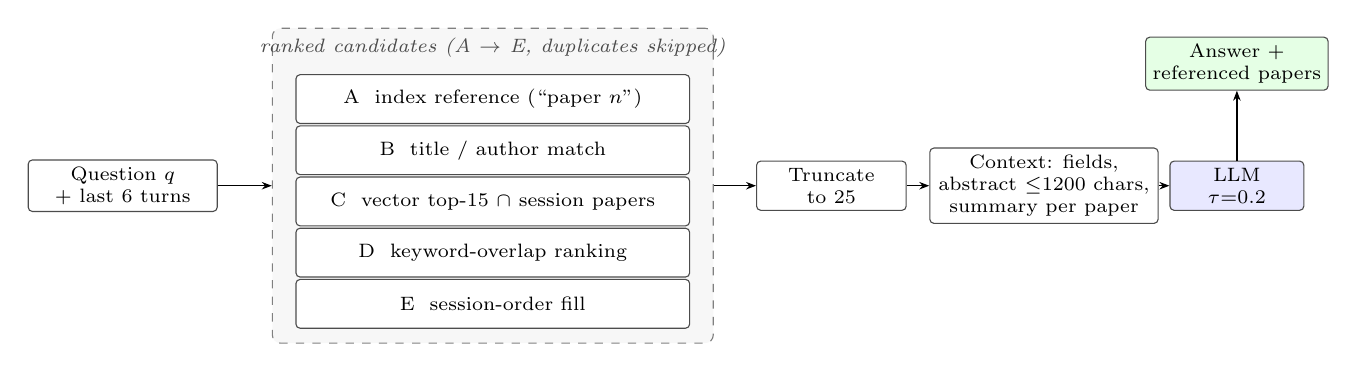
\begin{tikzpicture}[x=1cm,y=1cm]
\node[blk,minimum width=2.4cm] (qq) at (1.3,1.6) {Question $q$\\+ last 6 turns};
\begin{scope}[on background layer]
\node[draw=black!50,dashed,rounded corners=3pt,fill=black!3,minimum width=5.6cm,minimum height=4.0cm] (box) at (6.0,1.6) {};
\end{scope}
\node[lab] at (6.0,3.35) {ranked candidates (A $\rightarrow$ E, duplicates skipped)};
\node[blk,minimum width=5.0cm] (sa) at (6.0,2.7) {A\ \ index reference (``paper $n$'')};
\node[blk,minimum width=5.0cm] (sb) at (6.0,2.05) {B\ \ title / author match};
\node[blk,minimum width=5.0cm] (sc) at (6.0,1.4) {C\ \ vector top-15 $\cap$ session papers};
\node[blk,minimum width=5.0cm] (sd) at (6.0,0.75) {D\ \ keyword-overlap ranking};
\node[blk,minimum width=5.0cm] (se) at (6.0,0.1) {E\ \ session-order fill};
\node[blk,minimum width=1.9cm] (cap) at (10.3,1.6) {Truncate\\to 25};
\node[blk,minimum width=2.9cm] (ctx) at (13.0,1.6) {Context: fields,\\abstract $\le$1200 chars,\\summary per paper};
\node[blk,minimum width=1.7cm,fill=blue!9] (llm) at (15.45,1.6) {LLM\\$\tau{=}0.2$};
\node[blk,minimum width=2.0cm,fill=green!10] (ans2) at (15.45,3.15) {Answer +\\referenced papers};
\draw[arr] (qq) -- (box.west |- qq);
\draw[arr] (box.east |- cap) -- (cap);
\draw[arr] (cap) -- (ctx); \draw[arr] (ctx) -- (llm);
\draw[arr] (llm) -- (ans2);
\end{tikzpicture}
\caption{Hybrid evidence selection. Stages are ordered by specificity so that explicit references are never displaced by weaker topical matches.}
\label{fig:qa}
\end{figure*}

\section{Cross-Cutting Systems Concerns}
\label{sec:sys}

\subsection{Implementation Stack}
The service is written in Python. A FastAPI \cite{fastapi} application exposes the interface; the state machine is compiled with LangGraph \cite{langgraph} and checkpointed to SQLite; paper embeddings are held in a persistent Chroma \cite{chroma} collection; the graph uses NetworkX \cite{hagberg2008networkx}; PDF text is extracted with PyMuPDF \cite{pymupdf}; and reports are rendered with ReportLab and python-docx. The LLM is a Gemini Flash-class model reached through the vendor SDK, and the whole LLM interface is a single function taking a prompt, a system role, a token budget, and a temperature, which isolates the provider from every agent.

\subsection{Concurrency and Cost Bound}
Table~\ref{tab:ops} lists the parallelism and LLM usage of each stage. Parallel units write to index-addressed slots, so output order equals input order regardless of completion order. Because the control graph is acyclic and no stage loops on LLM output, the number of LLM calls per run is bounded by
\begin{equation}
N_{\mathrm{LLM}}\le\underbrace{1}_{\text{plan}}+\underbrace{2n}_{\text{extract}}+\underbrace{n}_{\text{synth}}+\underbrace{1}_{\text{cluster}}+\underbrace{2+|\Gamma|}_{\text{report}}=3n+|\Gamma|+4,
\label{eq:calls}
\end{equation}
where $n=|\cP|\le120$ and $|\Gamma|\le K\le5$, giving at most $369$ calls independent of what the model returns.

\begin{table}[!t]
\caption{Parallelism and LLM usage per stage.}
\label{tab:ops}
\centering
\small
\setlength{\tabcolsep}{3.5pt}
\begin{tabular}{@{}llccc@{}}
\toprule
Stage & Parallel unit & Workers & LLM calls & Temp. \\
\midrule
Planner    & --                      & 1   & 1            & 0 \\
Search     & (source, sub-query)     & 6   & 0            & -- \\
Extraction & paper                   & 8   & 1--2 / paper & 0 / 0.1 \\
Synthesis  & paper                   & 8   & 1 / paper    & 0 \\
Graph/Gap  & --                      & 1   & 1            & 0 \\
Report     & section / gap           & 2 / 5 & $2+|\Gamma|$ & 0.2 \\
Q\&A       & --                      & 1   & 1 / question & 0.2 \\
\bottomrule
\end{tabular}
\end{table}

\subsection{Caching and Retry}
Every search response is cached in a file keyed by the MD5 digest of a canonical JSON serialisation of the call arguments, prefixed by the source name. A hit is valid for a source-specific time to live: 30 days for arXiv metadata, which is close to immutable, and 3 days for the bibliographic API, whose citation counts change faster (7 days for any other prefix). A miss in the local cache consults a bundled offline snapshot whose entries never expire, and only then calls the live API. Entries written before the timestamped format was introduced are treated as expired. Transient failures are retried with exponential back-off,
\begin{equation}
d_i=d_0\,2^{\,i},\quad i=0,\dots,r-1,\qquad D_{\max}=d_0(2^{r}-1),
\label{eq:backoff}
\end{equation}
with $(d_0,r)=(2\,\mathrm{s},3)$ for arXiv ($D_{\max}=14$\,s) and $(3\,\mathrm{s},5)$ for the bibliographic API ($D_{\max}=93$\,s). Only rate-limit responses and transient network errors (connection, timeout, 502, 503) are retried; other errors fail immediately. After the last attempt the call returns an empty list, which the retrieval stage treats as a soft failure.

\subsection{Job Lifecycle, Persistence, Cancellation, and Access Control}
Submitting a topic creates a UUID job, spawns the pipeline as a background task, and returns the identifier at once. Status, results, and Q\&A are served from an in-memory job registry. For authenticated users the finished result bundle (papers, table, summaries, gaps, sub-queries, report draft) is also written as JSON to a relational store, and a request for a job that is missing from memory restores it from that store, which makes finished reviews survive a restart. Anonymous jobs live only in memory. Accounts use bcrypt-hashed passwords and HS256-signed bearer tokens with a seven-day default lifetime; the submission endpoint accepts requests with or without a token, while history endpoints require one.

Cancellation is cooperative. A cancel request adds the job to a flag set, and the flag is consulted at the start of the job, after retrieval, in the completion loops of extraction and synthesis, in the downstream agents (which short-circuit when an upstream agent is cancelled), and after the graph returns. It does not interrupt an in-flight network or LLM call.

\subsection{Degradation Hierarchy and Provenance}
Table~\ref{tab:degrade} lists the behaviour of every dependency on failure. Two job-level flags (mock-mode and embeddings-degraded), a per-gap signal-degraded flag, and the per-field verification status and abstract-only flag let a consumer see exactly which fallbacks fired. When no LLM credential is configured, the LLM client returns deterministic responses selected by prompt pattern; this keeps the pipeline testable offline, but its outputs are placeholders and the job is marked accordingly.

\begin{table}[!t]
\caption{Failure behaviour and provenance signal per dependency.}
\label{tab:degrade}
\centering
\small
\begin{tabular}{@{}>{\raggedright\arraybackslash}p{1.7cm}>{\raggedright\arraybackslash}p{2.55cm}>{\raggedright\arraybackslash}p{2.95cm}@{}}
\toprule
Component & On failure & Visible signal \\
\midrule
LLM service & deterministic pattern-matched responses & job mock-mode flag \\
Planner & $\cQ=\{q_0\}$ & agent status \textit{error} \\
Search APIs & empty result for that call (partial corpus) & log only \\
PDF & abstract-only prompt & abstract-only flag \\
Extraction & rule-based record & status \textit{heuristic} \\
Embeddings & pseudo-random vectors & job and per-gap degraded flags \\
Clustering & keyword clusters & log only \\
Gap stage & skipped if $|\cP|<15$ & empty $\Gamma$ \\
Report & template text & log only \\
\bottomrule
\end{tabular}
\end{table}

\section{Component-Level Evaluation}
\label{sec:eval}

\subsection{Scope and Setup}
No LLM credential was available, so the LLM-dependent qualities (extraction accuracy, summary faithfulness, report quality) are \emph{not} evaluated here. We instead evaluate the deterministic components through the implemented functions, on a single CPU core: (B) the deduplication tier on a snapshot of 90 raw records (45 arXiv, 45 bibliographic-API) from the bundled offline cache for three sub-queries on one topic; (C) the grounding verifier on quotes drawn from that snapshot's abstracts; (D) the gap detector on synthetic corpora with planted structure, running the complete implemented routine including its permutation null and replacing only the graph builder and the LLM clustering by deterministic stubs; and (E) orchestration and graph probes. The project's own suite of 25 automated tests (24 unit, 1 integration) also passes. Binomial proportions carry 95\% Wilson intervals \cite{wilson1927}.

\subsection{Deduplication}
The 90 raw records reduce to 83 unique papers (38 arXiv, 45 bibliographic; 63 with a PDF link; years 2017--2026). All seven removed duplicates matched on arXiv identifier, i.e., the same arXiv paper returned for different sub-queries. The two sources returned disjoint papers in this snapshot, so it does not exercise the cross-source merge path, even though 25 of the 45 bibliographic records carry an arXiv identifier. Among the 3\,403 pairs of retained papers the largest title Jaccard similarity is 0.63.

To probe the approximate-title tier alone we perturbed each retained title. At $\tau_J=0.8$ recall is $100\%$ for case and punctuation changes ($n{=}83$), $98.8\%$ for one inserted word, $97.6\%$ for one dropped word, $55.6\%$ for two, $13.9\%$ for three, and $0\%$ when a subtitle is removed ($n{=}40$). Table~\ref{tab:dedup} sweeps the threshold, pooling the word-insertion and word-drop perturbations. At $\tau_J\le0.6$ two distinct pairs would be merged wrongly, including consecutive parts of a series; at $0.7$ and above none are. The deployed $0.8$ is therefore conservative: it produced no false merge here, at the price of missing titles that differ by two or more words, which the identifier tiers recover when identifiers exist.

\begin{table}[!t]
\caption{Title-tier threshold sweep (perturbation recall pooled over four perturbation types; false merges among the 3\,403 distinct pairs).}
\label{tab:dedup}
\centering
\small
\begin{tabular}{@{}lccccc@{}}
\toprule
$\tau_J$ & 0.5 & 0.6 & 0.7 & \textbf{0.8} & 0.9 \\
\midrule
Recall (\%) & 99.4 & 95.7 & 85.8 & \textbf{68.0} & 35.1 \\
False-merge pairs & 2 & 2 & 0 & \textbf{0} & 0 \\
\bottomrule
\end{tabular}
\end{table}

\subsection{Grounding Verifier}
\textbf{Protocol.} Quotes are sentences of 40--330 characters. The verification text is a 12\,000-character window assembled from half of the abstracts, a size comparable to the LLM prompt window. True quotes come from inside the window. Fabricated quotes are sentences from the \emph{other} half of the abstracts, so they share vocabulary with the window, which makes them a deliberately hard negative. True quotes are corrupted at a character-noise rate $\eta$ split evenly into deletions, substitutions, and insertions, emulating text-extraction noise.

\textbf{Results.} Table~\ref{tab:ground} and Fig.~\ref{fig:results}a show that for quotes under 200 characters (the larger stratum in our sample, 60 of 74 true quotes) the verifier accepts $91.7\%$ of true quotes at $\eta=5\%$ and $83.3\%$ at $10\%$; at $\eta\ge20\%$ they move to \textit{unverified} but are almost never \textit{failed} ($\le3.3\%$ up to $\eta=40\%$). None of the 60 fabricated quotes was verified: $85\%$ were \textit{failed} and $15\%$ \textit{unverified}, with a maximum score of $0.58$, which is $0.27$ below the acceptance threshold. The average cost is about $0.18$\,s per short quote on this window.

\textbf{Long quotes.} For quotes of 200 characters or more ($n{=}14$) the implemented matcher behaves very differently: at $\eta=5\%$ only $7.1\%$ are verified and $35.7\%$ are \textit{failed}. Disabling the string-matching library's automatic ``junk'' heuristic, which engages for sequences of 200 or more items, restores $92.9\%$ verified and $0\%$ failed, at $4.7\times$ the cost ($0.27$\,s versus $0.058$\,s per quote). We return to this in Section~\ref{sec:disc}. As a sanity check of the abstract-only rule, values built from three words of the paper's own abstract were verified in $56/56$ cases and values built from three words of another paper's abstract in $0/56$; this checks that the rule implements keyword presence, not extraction quality.

\begin{table}[!t]
\caption{Verifier outcome (\%) for true quotes under noise rate $\eta$, and for fabricated quotes. Long = quotes of at least 200 characters.}
\label{tab:ground}
\centering
\footnotesize
\setlength{\tabcolsep}{3.5pt}
\begin{tabular}{@{}llccc@{}}
\toprule
Quotes & Setting & Verified & Unverif. & Failed \\
\midrule
\multirow{6}{*}{Short ($n{=}60$)} & $\eta=0.00$ & 100.0 & 0.0 & 0.0 \\
 & $\eta=0.05$ & 91.7 & 8.3 & 0.0 \\
 & $\eta=0.10$ & 83.3 & 16.7 & 0.0 \\
 & $\eta=0.20$ & 13.3 & 86.7 & 0.0 \\
 & $\eta=0.30$ & 0.0 & 98.3 & 1.7 \\
 & $\eta=0.40$ & 0.0 & 96.7 & 3.3 \\
\midrule
Fabricated ($n{=}60$) & -- & 0.0 & 15.0 & 85.0 \\
\midrule
\multirow{2}{*}{Long ($n{=}14$)} & $\eta=0.05$, default & 7.1 & 57.1 & 35.7 \\
 & $\eta=0.05$, junk off & 92.9 & 7.1 & 0.0 \\
\bottomrule
\end{tabular}
\end{table}

\subsection{Gap Detector}
\textbf{Protocol.} Each synthetic corpus has $n=60$ papers in $K=4$ planted clusters of sizes $18,16,14,12$ with publication years uniform in 2016--2025. Similarity edges occur with probability $0.25$ inside a cluster and $0.06$ across clusters; a citation edge $i\to j$ ($y_i\ge y_j$) occurs with probability $0.05$ inside and $0.02$ across clusters, multiplied by a deficit factor $\delta$ when $j$ lies in the \emph{target} cluster (size 12). The LLM clustering is stubbed with the planted clusters, so the experiment evaluates the statistical detector rather than the clustering. We report $P(\text{target flagged})$ and the false-flag rate on the other clusters.

\begin{table}[!t]
\caption{Gap detector on synthetic corpora ($T{=}300$ trials per row unless stated; 95\% Wilson intervals).}
\label{tab:gap}
\centering
\footnotesize
\setlength{\tabcolsep}{3.5pt}
\begin{tabular}{@{}lcc@{}}
\toprule
Condition & $P$(target flagged) & Other clusters \\
\midrule
Null: random membership & 10.1\ [9.1, 11.0]$^{\ast}$ & -- \\
\midrule
Citation factor $\delta=1.0$ & 11.7\ [8.5, 15.8] & 11.4 \\
$\delta=0.6$ & 24.7\ [20.1, 29.8] & 4.6 \\
$\delta=0.3$ & 26.3\ [21.7, 31.6] & 0.8 \\
$\delta=0.1$ & 25.3\ [20.7, 30.5] & 0.2 \\
\midrule
Cross-sim.\ $0.01$ ($\delta{=}0.3$) & 0.0\ [0.0, 1.3] & 1.0 \\
Cross-sim.\ $0.06$ ($\delta{=}0.3$) & 24.7\ [20.1, 29.8] & 1.3 \\
Cross-sim.\ $0.15$ ($\delta{=}0.3$) & 98.0\ [95.7, 99.1] & 0.0 \\
\bottomrule
\multicolumn{3}{@{}l}{\scriptsize $^{\ast}$Per-cluster rate over all clusters, $T{=}1000$. Values in \%.}
\end{tabular}
\end{table}

\begin{figure*}[!t]
\centering
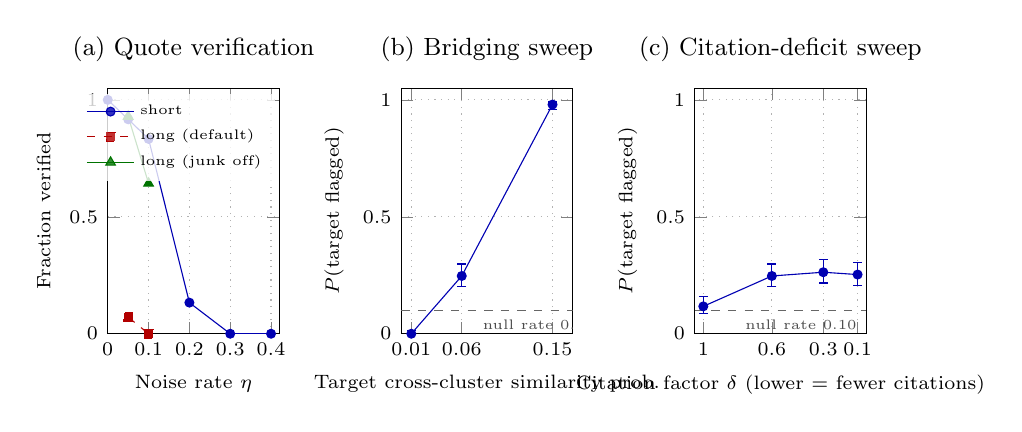
\begin{tikzpicture}
\begin{groupplot}[group style={group size=3 by 1,horizontal sep=1.55cm},width=0.31\textwidth,height=4.7cm,
  tick label style={font=\scriptsize},label style={font=\scriptsize},title style={font=\small},
  legend style={font=\tiny,draw=none,fill=none},grid=major,grid style={dotted,black!30}]
\nextgroupplot[title={(a) Quote verification},xlabel={Noise rate $\eta$},ylabel={Fraction verified},
  xmin=0,xmax=0.42,ymin=0,ymax=1.05,legend style={at={(0.98,0.98)},anchor=north east,font=\tiny,draw=none,fill=white,fill opacity=0.8,text opacity=1},legend cell align=left]
\addplot[blue!70!black,mark=*,mark size=1.6pt] coordinates {(0,1)(0.05,0.917)(0.10,0.833)(0.20,0.133)(0.30,0)(0.40,0)};
\addplot[red!70!black,mark=square*,mark size=1.6pt,dashed] coordinates {(0.05,0.071)(0.10,0)};
\addplot[green!45!black,mark=triangle*,mark size=2pt] coordinates {(0.05,0.929)(0.10,0.643)};
\legend{short,long (default),long (junk off)}
\nextgroupplot[title={(b) Bridging sweep},xlabel={Target cross-cluster similarity prob.},ylabel={$P$(target flagged)},
  xmin=0,xmax=0.17,ymin=0,ymax=1.05,xtick={0.01,0.06,0.15},scaled x ticks=false,xticklabel style={/pgf/number format/fixed,/pgf/number format/precision=2}]
\addplot[blue!70!black,mark=*,mark size=1.6pt,error bars/.cd,y dir=both,y explicit]
  table[row sep=\\,y error plus=ep,y error minus=em]{x y ep em\\ 0.01 0.0 0.013 0.0\\ 0.06 0.247 0.051 0.046\\ 0.15 0.980 0.011 0.023\\};
\draw[dashed,black!60] (axis cs:0,0.10) -- (axis cs:0.17,0.10) node[pos=0.80,below,font=\tiny,text=black!70]{null rate 0.10};
\nextgroupplot[title={(c) Citation-deficit sweep},xlabel={Citation factor $\delta$ (lower $=$ fewer citations)},ylabel={$P$(target flagged)},
  xmin=0.05,xmax=1.05,ymin=0,ymax=1.05,x dir=reverse,xtick={1.0,0.6,0.3,0.1}]
\addplot[blue!70!black,mark=*,mark size=1.6pt,error bars/.cd,y dir=both,y explicit]
  table[row sep=\\,y error plus=ep,y error minus=em]{x y ep em\\ 1.0 0.117 0.041 0.032\\ 0.6 0.247 0.051 0.046\\ 0.3 0.263 0.053 0.046\\ 0.1 0.253 0.052 0.046\\};
\draw[dashed,black!60] (axis cs:1.05,0.10) -- (axis cs:0.05,0.10) node[pos=0.62,below,font=\tiny,text=black!70]{null rate 0.10};
\end{groupplot}
\end{tikzpicture}
\caption{(a) Fraction of true quotes verified versus character-noise rate; ``long'' quotes have 200 or more characters ($n{=}14$). (b),(c) Probability that the planted target cluster is flagged; bars are 95\% Wilson intervals, dashed line is the nominal null rate.}
\label{fig:results}
\end{figure*}

\textbf{Calibration.} Under random membership the per-cluster flag rate is $10.05\%$ (half-width $0.93$ points), matching the nominal $10\%$. Because $K=4$ clusters are tested, the chance that a run flags at least one is $39.2\%$ ($608$ of $1000$ runs flagged none, $382$ one, $10$ two): the per-cluster guarantee does not carry over to the run.

\textbf{Sensitivity.} Raising the target's cross-cluster similarity from $0.06$ to $0.15$ lifts $P$(flag) from $24.7\%$ to $98.0\%$, whereas lowering it to $0.01$ yields $0.0\%$, consistent with the sign of Eq.~\eqref{eq:score}: the detector rewards bridging (Fig.~\ref{fig:results}b). A citation deficit alone raises $P$(flag) from $11.7\%$ (no deficit, close to the null) to about $25\%$ at $\delta=0.6$ and then saturates, even at a tenfold deficit (Fig.~\ref{fig:results}c); false flags on the other clusters fall from $11.4\%$ to $0.2\%$. A low pace is thus necessary but not sufficient, because the min--max-normalised pace term contributes at most one unit and the score is also gated by bridging. The configuration $\delta=0.3$, cross-similarity $0.06$ appears in both sweeps as independent replicates ($26.3\%$ and $24.7\%$).

\textbf{Degenerate regimes.} With no similarity edges, as in the degraded-embedding mode, exactly one cluster was flagged in $149$ of $150$ trials: every null score is $\le0$ and at least one in $K$ equals $0$, so $\theta=0$ and the non-strict test passes the lowest-pace cluster by construction. With no edges at all, all four clusters were flagged in $40$ of $40$ trials.

\subsection{Orchestration and Real-Graph Probes}
\textbf{Progress visibility.} A probe confirmed that a status map mutated in place by a node is observed by the holder of the original reference while the graph runs, as Section~\ref{sec:arch} assumes.

\textbf{Job identifier.} The job identifier is set in the initial state but is not declared in the state schema. With LangGraph 1.2.12 an undeclared key is dropped from node inputs: in a run of the compiled graph with stubbed network and file output, all six agents observed a null identifier, and a cancellation flag raised \emph{before} invocation did not stop any agent (all reached \textit{done}).

\textbf{Citation edges on real data.} On the 83-paper snapshot the graph builder (embedding service disabled) creates 352 authorship and 1\,664 co-authorship edges and \emph{no} citation edge. Thirty-eight papers carry citation lists totalling 3\,452 identifiers, all of them bibliographic-service identifiers, whereas the corpus identifiers are 42 DOIs, 38 arXiv identifiers, and 3 service identifiers; no list entry matches a corpus identifier. In addition, the list length equals the reported citation count for 36 of 38 papers and never exceeds it, which indicates that the lists enumerate \emph{citing} papers (incoming citations) rather than references.

\section{Discussion and Limitations}
\label{sec:disc}
The evaluation exposes eight limitations of the current implementation. Each has a local remedy.

\textbf{L1: Citation edges are not formed on real data.} The membership test compares service-specific identifiers with a canonical identifier space that is mostly DOIs and arXiv identifiers, so $E_{\mathrm{cite}}=\varnothing$ on the real snapshot; and the stored lists are incoming, so an edge $(p,q)$ built from $q\in L_p$ would read ``$p$ cites $q$'' when the data say ``$q$ cites $p$''. With $E_{\mathrm{cite}}=\varnothing$ we get $\pi_k=0$ for all $k$, the corpus-too-recent branch fires, and the gap score reduces to the bridging term alone. \emph{Remedy:} keep the service identifier on each paper record, resolve list entries through it, and reverse the edge direction (or request reference lists). This is the most consequential limitation, because it affects the headline signal; the synthetic experiments of Section~\ref{sec:eval}-D test the detector given correct edges.

\textbf{L2: Length-dependent matcher bias.} Quotes of 200 or more characters are under-verified (Section~\ref{sec:eval}-C). \emph{Remedy:} disable the junk heuristic, accepting a $4.7\times$ cost increase, or constrain the prompt to request short quotations.

\textbf{L3: Ties flag everything.} The non-strict threshold together with min--max normalisation makes the detector flag the lowest-pace cluster, or all clusters, when evidence is absent. \emph{Remedy:} use a strict inequality and return an ``insufficient evidence'' status when both signals are constant or the graph lacks citation or similarity edges.

\textbf{L4: No multiplicity control.} Per-cluster calibration yields a 39\% run-level false-flag probability for $K=4$. \emph{Remedy:} compare each $s_k$ with the null distribution of the per-replicate maximum, or control the false-discovery rate \cite{benjamini1995fdr}.

\textbf{L5: Uneven sensitivity.} In our synthetic setting the score responds strongly to bridging and weakly to citation deficit. Whether this matches the intended notion of a gap should be settled by expert review.

\textbf{L6: Unseeded null.} The permutation null draws from a process-global random generator without a seed, so the threshold, and hence a borderline flag, can differ between runs. \emph{Remedy:} seed per job and increase $R$.

\textbf{L7: Presence is not entailment.} The verifier establishes that a quotation occurs in the text, not that it supports the extracted value; a quotation from a related-work sentence would pass. The abstract-only rule is keyword-level. \emph{Remedy:} add an entailment check between quote and value.

\textbf{L8: Cancellation and log tagging.} Because of the dropped job identifier (Section~\ref{sec:eval}-E) the in-agent cancellation checkpoints and job-tagged logging are inactive; cancellation takes effect only before launch and after completion. \emph{Remedy:} declare the key in the state schema.

\textbf{Threats to validity.} The deduplication snapshot covers one topic and three sub-queries; the long-quote stratum has $n{=}14$; the gap experiments are synthetic and use planted, correct clusters; and no end-to-end, human-judged evaluation of extraction, summarisation, or gap relevance was possible. The deterministic mock responses used when no LLM is configured are plumbing stubs and should not be read as a baseline.

\section{Conclusion}
\label{sec:concl}
\RM\ shows that a literature-review assistant can be built as a fixed, resumable, six-stage pipeline in which the LLM is bracketed by verification, fallbacks, and provenance flags. Its two analytical components are explicit and inspectable: a fuzzy-quote verifier with a four-valued status, and a gap score that combines age-adjusted citation pace with cross-cluster bridge strength under a permutation null. Measurements on the implemented code confirm that the verifier separates fabricated from genuine short quotations with a margin and that the gap threshold is calibrated per cluster, and they pinpoint the changes needed before the citation signal can be trusted on real data: identifier resolution and edge direction, strict tie handling, and multiplicity control. Future work comprises these fixes, an endpoint that exposes checkpoint resume, entailment-based verification, and a human-judged evaluation of extraction accuracy, summary faithfulness, and the relevance of the flagged gaps.

\balance
\begin{thebibliography}{99}
\bibitem{fortunato2018science} S. Fortunato \emph{et al.}, ``Science of science,'' \emph{Science}, vol. 359, no. 6379, p. eaao0185, 2018.
\bibitem{ji2023hallucination} Z. Ji \emph{et al.}, ``Survey of hallucination in natural language generation,'' \emph{ACM Comput. Surv.}, vol. 55, no. 12, pp. 1--38, 2023.
\bibitem{lewis2020rag} P. Lewis \emph{et al.}, ``Retrieval-augmented generation for knowledge-intensive {NLP} tasks,'' in \emph{Proc. NeurIPS}, 2020.
\bibitem{yao2023react} S. Yao \emph{et al.}, ``{ReAct}: Synergizing reasoning and acting in language models,'' in \emph{Proc. ICLR}, 2023.
\bibitem{wu2023autogen} Q. Wu \emph{et al.}, ``{AutoGen}: Enabling next-gen {LLM} applications via multi-agent conversation,'' arXiv:2308.08155, 2023.
\bibitem{hong2024metagpt} S. Hong \emph{et al.}, ``{MetaGPT}: Meta programming for a multi-agent collaborative framework,'' in \emph{Proc. ICLR}, 2024.
\bibitem{langgraph} LangChain, ``{LangGraph}: Build resilient language agents as graphs.'' [Online]. Available: https://github.com/langchain-ai/langgraph
\bibitem{ratcliff1988gestalt} J. W. Ratcliff and D. E. Metzener, ``Pattern matching: The gestalt approach,'' \emph{Dr. Dobb's Journal}, vol. 13, no. 7, p. 46, 1988.
\bibitem{garfield1955citation} E. Garfield, ``Citation indexes for science,'' \emph{Science}, vol. 122, no. 3159, pp. 108--111, 1955.
\bibitem{small1973cocitation} H. Small, ``Co-citation in the scientific literature,'' \emph{J. Amer. Soc. Inf. Sci.}, vol. 24, no. 4, pp. 265--269, 1973.
\bibitem{wang2013quantifying} D. Wang, C. Song, and A.-L. Barab{\'a}si, ``Quantifying long-term scientific impact,'' \emph{Science}, vol. 342, no. 6154, pp. 127--132, 2013.
\bibitem{kinney2023s2} R. Kinney \emph{et al.}, ``The {Semantic Scholar} open data platform,'' arXiv:2301.10140, 2023.
\bibitem{arxivapi} arXiv, ``{arXiv API} user's manual.'' [Online]. Available: https://info.arxiv.org/help/api/
\bibitem{efron1979bootstrap} B. Efron, ``Bootstrap methods: Another look at the jackknife,'' \emph{Ann. Statist.}, vol. 7, no. 1, pp. 1--26, 1979.
\bibitem{phipson2010permutation} B. Phipson and G. K. Smyth, ``Permutation p-values should never be zero,'' \emph{Stat. Appl. Genet. Mol. Biol.}, vol. 9, no. 1, art. 39, 2010.
\bibitem{jaccard1912} P. Jaccard, ``The distribution of the flora in the alpine zone,'' \emph{New Phytologist}, vol. 11, no. 2, pp. 37--50, 1912.
\bibitem{reimers2019sbert} N. Reimers and I. Gurevych, ``{Sentence-BERT}: Sentence embeddings using {Siamese BERT}-networks,'' in \emph{Proc. EMNLP-IJCNLP}, 2019, pp. 3982--3992.
\bibitem{wilson1927} E. B. Wilson, ``Probable inference, the law of succession, and statistical inference,'' \emph{J. Amer. Statist. Assoc.}, vol. 22, no. 158, pp. 209--212, 1927.
\bibitem{benjamini1995fdr} Y. Benjamini and Y. Hochberg, ``Controlling the false discovery rate: A practical and powerful approach to multiple testing,'' \emph{J. R. Stat. Soc. B}, vol. 57, no. 1, pp. 289--300, 1995.
\bibitem{fastapi} S. Ram{\'i}rez, ``{FastAPI}.'' [Online]. Available: https://fastapi.tiangolo.com
\bibitem{chroma} Chroma, ``Chroma: The open-source embedding database.'' [Online]. Available: https://www.trychroma.com
\bibitem{hagberg2008networkx} A. A. Hagberg, D. A. Schult, and P. J. Swart, ``Exploring network structure, dynamics, and function using {NetworkX},'' in \emph{Proc. 7th Python in Science Conf. (SciPy)}, 2008, pp. 11--15.
\bibitem{pymupdf} Artifex Software, ``{PyMuPDF} documentation.'' [Online]. Available: https://pymupdf.readthedocs.io
\end{thebibliography}
\end{document}
